\pdfoutput=1
\documentclass[12pt]{article}
% Load preamble (packages, math, definitions, comments)
%\RequirePackage[l2tabu, orthodox]{nag}

% FONTS
\usepackage[utf8]{inputenc} % allow utf-8 input
\usepackage[T1]{fontenc}    % use 8-bit T1 fonts

% Replace default Latin Modern typewriter with its proportional counterpart
% http://www.tug.dk/FontCatalogue/lmoderntypewriterprop/
\renewcommand*\ttdefault{lmvtt}


%%% OPTION 1 - Fourier Math + New Century Schoolbook + ParaType Sans

% % Import Fourier Math (this imposes its own New Century Schoolbook type)
% % http://www.ctan.org/tex-archive/fonts/fouriernc/
% \usepackage{fouriernc}
% \usepackage{amsmath}
% % Replace with TeX Gyre Schola version of New Century Schoolbook (must scale!)
% % http://www.tug.dk/FontCatalogue/tgschola/
% \usepackage[scale=0.92]{tgschola}
% \usepackage[scaled=0.88]{PTSans}

%% OPTION 2 - MathDesign Math + Bitstream Charter + ParaType Sans

% Import MathDesign (this brings along Bitstream Charter)
% http://www.ctan.org/tex-archive/fonts/mathdesign/
\usepackage[bitstream-charter]{mathdesign}
\usepackage{amsmath}
\usepackage[scaled=0.92]{PTSans}


% %%% OPTION 3 - MTPRO 2 Math + Termes Times + ParaType Sans

% \usepackage{tgtermes}
% \usepackage{amsmath}
% \usepackage[subscriptcorrection,
%             amssymbols,
%             mtpbb,
%             mtpcal,
%             nofontinfo  % suppresses all warnings
%            ]{mtpro2}
% \usepackage{scalefnt,letltxmacro}
% \LetLtxMacro{\oldtextsc}{\textsc}
% \renewcommand{\textsc}[1]{\oldtextsc{\scalefont{1.10}#1}}
% \usepackage[scaled=0.92]{PTSans}

% GEOMETRY
\usepackage[
  paper  = letterpaper,
  left   = 1.0in,
  right  = 1.0in,
  top    = 1.0in,
  bottom = 1.0in,
  ]{geometry}

% COLOR
\usepackage[usenames,dvipsnames,table]{xcolor}
%\usepackage[usenames,table]{xcolor}
\definecolor{shadecolor}{gray}{0.9}

% SPACING and TEXT
\usepackage[final,expansion=alltext]{microtype}
\usepackage[english]{babel}
\usepackage[parfill]{parskip}
\usepackage{afterpage}
\usepackage{framed}

%redefine the leftbar environment to accept a width and coloring options
\renewenvironment{leftbar}[1][\hsize]
{%
  \def\FrameCommand
  {%
    {\color{Gray}\vrule width 3pt}%
    \hspace{10pt}%
    %\hspace{0pt}\fboxsep=\FrameSep\colorbox{black!10}%
  }%
  \MakeFramed{\hsize#1\advance\hsize-\width\FrameRestore}%
}%
{\endMakeFramed}

% define a paragraph header function
\DeclareRobustCommand{\parhead}[1]{\textbf{#1}~}

% EDITING
% line numbering in left margin
\usepackage{lineno}
\renewcommand\linenumberfont{\normalfont
                             \footnotesize
                             \sffamily
                             \color{SkyBlue}}
% ragged paragraphs in right margin
\usepackage{ragged2e}
\DeclareRobustCommand{\sidenote}[1]{\marginpar{
                                    \RaggedRight
                                    \textcolor{Plum}{\textsf{#1}}}}
% paragraph counter in right margin
\newcommand{\parnum}{\bfseries\P\arabic{parcount}}
\newcounter{parcount}
\newcommand\p{%
    \stepcounter{parcount}%
    \leavevmode\marginpar[\hfill\parnum]{\parnum}%
}
% paragraph helper
\DeclareRobustCommand{\PP}{\textcolor{Plum}{\P} }

% COUNTERS
\renewcommand{\labelenumi}{\color{black!67}{\arabic{enumi}.}}
\renewcommand{\labelenumii}{{\color{black!67}(\alph{enumii})}}
\renewcommand{\labelitemi}{{\color{black!67}\textbullet}}

% FIGURES
\usepackage{graphicx}
\usepackage{float}  % for the [H] float placement specifier
\usepackage{wrapfig}
\usepackage[labelfont=bf,font=footnotesize,width=.9\textwidth]{caption}
\usepackage[format=hang]{subcaption}

% TABLES
\usepackage{booktabs,multirow,multicol}       % professional-quality tables

% ALGORITHMS
\usepackage[algoruled]{algorithm2e}
\usepackage{listings}
\usepackage{fancyvrb}
\fvset{fontsize=\normalsize}

% BIBLIOGRAPHY
% Note: natbib is loaded in main.tex (after document class)
% For biblatex instead, use: \usepackage[%
minnames=1,maxnames=99,maxcitenames=2,
style=alphabetic,
doi=false,
url=false,
firstinits=true,
hyperref,
natbib,
backend=bibtex,
sorting=nyt
]{biblatex}%

\newbibmacro*{journal}{%
  \iffieldundef{journaltitle}
    {}
    {\printtext[journaltitle]{%
       \printfield[noformat]{journaltitle}%
       \setunit{\subtitlepunct}%
       \printfield[noformat]{journalsubtitle}}}}

\DeclareFieldFormat[article,inbook,incollection,inproceedings,patent,thesis,unpublished]{titlecase}{\MakeSentenceCase*{#1}}

\AtEveryBibitem{%
\ifentrytype{article}{
    \clearfield{url}%
    \clearfield{urldate}%
    \clearfield{eprint}
}{}
\ifentrytype{book}{
    \clearfield{url}%
    \clearfield{urldate}%
}{}
\ifentrytype{collection}{
    \clearfield{url}%
    \clearfield{urldate}%
}{}
\ifentrytype{incollection}{
    \clearfield{url}%
    \clearfield{urldate}%
}{}
}

\AtEveryBibitem{
    \clearfield{pages}
    \clearfield{review}%
    \clearfield{series}%%
    \clearfield{volume}
    \clearfield{pages}
    \clearfield{month}
    \clearfield{eprint}
    \clearfield{isbn}
    \clearfield{issn}
    \clearlist{location}
    \clearfield{series}
    \clearlist{publisher}
    \clearname{editor}
}{}

% HYPERREF
\usepackage[colorlinks,linktoc=all]{hyperref}
\usepackage[all]{hypcap}
\hypersetup{citecolor=MidnightBlue}
\hypersetup{linkcolor=MidnightBlue}
\hypersetup{urlcolor=MidnightBlue}

% CLEVEREF must come after HYPERREF
\usepackage[nameinlink,capitalise]{cleveref}
\Crefname{section}{\S}{\S}

% ACRONYMS
\usepackage[acronym,nowarn]{glossaries}
% Define an acronym style with small caps
\renewcommand*{\acronymfont}[1]{\textsc{#1}}

% COLOR DEFINITIONS
\newcommand{\red}[1]{\textcolor{BrickRed}{#1}}
\newcommand{\orange}[1]{\textcolor{BurntOrange}{#1}}
\newcommand{\green}[1]{\textcolor{OliveGreen}{#1}}
\newcommand{\blue}[1]{\textcolor{MidnightBlue}{#1}}
\newcommand{\gray}[1]{\textcolor{black!60}{#1}}

% LISTINGS DEFINTIONS
\lstdefinestyle{mystyle}{
    commentstyle=\color{OliveGreen},
    keywordstyle=\color{BurntOrange},
    numberstyle=\tiny\color{black!60},
    stringstyle=\color{MidnightBlue},
    basicstyle=\ttfamily,
    breakatwhitespace=false,
    breaklines=true,
    captionpos=b,
    keepspaces=true,
    numbers=left,
    numbersep=5pt,
    showspaces=false,
    showstringspaces=false,
    showtabs=false,
    tabsize=2
}
\lstset{style=mystyle}

% MATH PACKAGES AND DEFINITIONS
% !TEX root = main.tex

% MATH PACKAGES
% Note: amsfonts conflicts with mathdesign (loaded in preamble.tex)
% mathdesign provides its own blackboard bold, so we skip amsfonts
\usepackage{centernot}
\usepackage{amsthm}         % theorem environments
\usepackage{nicefrac}       % compact symbols for 1/2, etc.
\usepackage{mathtools}      % extends amsmath
\usepackage{amsbsy}         % bold math symbols
\usepackage{amstext}        % text in math mode
\usepackage{thmtools}       % theorem tools
\usepackage{thm-restate}    % restatable theorems

% compatibility w/ parskip https://tex.stackexchange.com/questions/25346/wrong-spacing-before-theorem-environment-amsthm
\begingroup
    \makeatletter
    \@for\theoremstyle:=definition,remark,plain\do{%
        \expandafter\g@addto@macro\csname th@\theoremstyle\endcsname{%
            \addtolength\thm@preskip\parskip
            }%
        }
\endgroup

\DeclareRobustCommand{\mb}[1]{\ensuremath{\mathbf{\boldsymbol{#1}}}}
% \DeclareRobustCommand{\mb}[1]{\mathbold{#1}}

\DeclareRobustCommand{\KL}[2]{\ensuremath{\textrm{KL}\left(#1\;\|\;#2\right)}}

% \DeclareMathOperator*{\argmax}{arg\,max}
% \DeclareMathOperator*{\argmin}{arg\,min}

\crefname{lemma}{lemma}{lemmas}
\Crefname{lemma}{Lemma}{Lemmas}
\crefname{thm}{theorem}{theorems}
\Crefname{thm}{Theorem}{Theorems}
\crefname{prop}{proposition}{propositions}
\Crefname{prop}{Proposition}{Propositions}
\crefname{assumption}{assumption}{assumptions}
\crefname{assumption}{Assumption}{Assumptions}


% \newtheorem{thm}{Theorem} % reset theorem numbering for each chapter
% \newtheorem{defn}{Definition} % definition numbers are dependent on theorem numbers
% \newtheorem{prop}[thm]{Proposition}
% \newtheorem{exmp}[thm]{Example} % same for example numbers
% \newtheorem{lemma}[thm]{Lemma}
% \newtheorem{assumption}{Assumption}
% \newtheorem{corollary}[thm]{Corollary}
% Independence symbol (double perp): use \indpt
\def\independenT#1#2{\mathrel{\rlap{$#1#2$}\mkern2mu{#1#2}}}



\def\checkmark{\tikz\fill[scale=0.4](0,.35) -- (.25,0) -- (1,.7) -- (.25,.15) -- cycle;} 

% Note: booktabs loaded in preamble.tex; arydshln adds dashed lines
\usepackage{arydshln}
\makeatletter
\def\adl@drawiv#1#2#3{%
        \hskip.5\tabcolsep
        \xleaders#3{#2.5\@tempdimb #1{1}#2.5\@tempdimb}%
                #2\z@ plus1fil minus1fil\relax
        \hskip.5\tabcolsep}
\newcommand{\cdashlinelr}[1]{%
  \noalign{\vskip\aboverulesep
           \global\let\@dashdrawstore\adl@draw
           \global\let\adl@draw\adl@drawiv}
  \cdashline{#1}
  \noalign{\global\let\adl@draw\@dashdrawstore
           \vskip\belowrulesep}}
\makeatother

\newenvironment{proofsk}{%
  \renewcommand{\proofname}{Proof sketch}\proof}{\endproof}

\renewcommand{\epsilon}{\varepsilon}

%********************************************************************
% Extra theorem environments
%********************************************************************

\declaretheorem[style=plain,numberwithin=section,name=Theorem]{theorem}
\declaretheorem[style=plain,sibling=theorem,name=Lemma]{lemma}
\declaretheorem[style=plain,sibling=theorem,name=Proposition]{proposition}
\declaretheorem[style=plain,sibling=theorem,name=Corollary]{cor}
\declaretheorem[style=plain,sibling=theorem,name=Claim]{claim}
\declaretheorem[style=plain,sibling=theorem,name=Conjecture]{conj}
\declaretheorem[style=definition,sibling=theorem,name=Definition]{defn}
\declaretheorem[style=definition,name=Assumption]{assumption}
\declaretheorem[style=definition,sibling=theorem,name=Example]{example}
\declaretheorem[style=remark,sibling=theorem,name=Remark]{remark}

\newenvironment{example*}
 {\pushQED{\qed}\example}
 {\popQED\endexample}
\numberwithin{equation}{section}

% This file contains definitions of custom macros
% ------------------------------------------------------------------------------

\newcommand{\grad}{\nabla}
\newcommand\dif{\mathop{}\!\mathrm{d}}
\newcommand{\diag}{\textrm{diag}}
\newcommand{\supp}{\textrm{supp}}
\newcommand{\E}[2]{\mathbb{E}_{#1}\left[#2\right]}
\newcommand{\G}[2]{\mathbb{G}_{#1}\left[#2\right]}
\newcommand{\V}[2]{\mathbb{V}_{#1}\left[#2\right]}

\newcommand{\defeq}{\overset{\mathrm{def}}{=}}
\newcommand{\equalas}{\overset{\mathrm{a.s.}}{=}}
\newcommand{\disteq}{\overset{d}{=}}
\newcommand{\iidsim}{\overset{\mathrm{iid}}{\sim}}
\newcommand{\indsim}{\overset{\mathrm{ind}}{\sim}}

\newcommand{\Reals}{\mathbb{R}}
\newcommand{\Nats}{\mathbb{N}}
\newcommand{\NNReals}{\Reals_{+}}

\newcommand{\exclude}{\backslash}

\newcommand{\eps}{\varepsilon}

\DeclareMathOperator*{\argmin}{argmin}
\DeclareMathOperator*{\argmax}{argmax}
\DeclareMathOperator*{\logit}{logit}

\newcommand{\abs}[1]{\left\lvert#1 \right\rvert}

%%% Local Variables:
%%% mode: latex
%%% TeX-master: "main"
%%% End:


% DRAFT COMMENTS (switch to nocommenting for production)
%%%%%%%%%%%%%%%%%%%%%%%%%%%%%%%%%%%%%%%%%%%%%%%%%%%%%%%%%%
%%%% EDITING HELPER FUNCTIONS  %%%%%%%%%%%%%%%%%%%%%%%%%%%
%%%%%%%%%%%%%%%%%%%%%%%%%%%%%%%%%%%%%%%%%%%%%%%%%%%%%%%%%%

%% NA: needs attention (rough writing whose correctness needs to be verified)
%% TBD: instructions for how to fix a gap ("Describe the propagation by ...")
%% PROBLEM: bug or missing crucial bit 

%% use \fXXX versions of these macros to put additional explanation into a footnote.  
%% The idea is that we don't want to interrupt the flow of the paper or make it 
%% impossible to read because there are a bunch of comments.

%% NA's (and TBDs, those less crucially) should be written so 
%% that they flow with the text.

\definecolor{WowColor}{rgb}{.75,0,.75}
\definecolor{SubtleColor}{rgb}{0,0,.50}

% inline
\newcommand{\NA}[1]{\textcolor{SubtleColor}{ {\tiny \bf ($\star$)} #1}}
\newcommand{\LATER}[1]{\textcolor{SubtleColor}{ {\tiny \bf ($\dagger$)} #1}}
\newcommand{\TBD}[1]{\textcolor{SubtleColor}{ {\tiny \bf (!)} #1}}
\newcommand{\PROBLEM}[1]{\textcolor{WowColor}{ {\bf (!!)} {\bf #1}}}

% as margin notes

\newcounter{margincounter}
\newcommand{\displaycounter}{{\arabic{margincounter}}}
\newcommand{\incdisplaycounter}{{\stepcounter{margincounter}\arabic{margincounter}}}

\newcommand{\fTBD}[1]{\textcolor{SubtleColor}{$\,^{(\incdisplaycounter)}$}\marginpar{\raggedright\tiny\textcolor{SubtleColor}{ {\tiny $(\displaycounter)$} #1}}}

\newcommand{\fPROBLEM}[1]{\textcolor{WowColor}{$\,^{((\incdisplaycounter))}$}\marginpar{\raggedright\tiny\textcolor{WowColor}{ {\bf $\mathbf{((\displaycounter))}$} {\bf #1}}}}

\newcommand{\fLATER}[1]{\textcolor{SubtleColor}{$\,^{(\incdisplaycounter\dagger)}$}\marginpar{\raggedright\tiny\textcolor{SubtleColor}{ {\tiny $(\displaycounter\dagger)$} #1}}}

% % Production mode: error on leftover draft comments
% Switch to commenting.tex during drafting

\newcommand{\LATER}[1]{\PackageError{nocommenting}{Leftover LATER comment}{Remove all LATER comments before final build}}
\newcommand{\fLATER}[1]{\PackageError{nocommenting}{Leftover fLATER comment}{Remove all fLATER comments before final build}}
\newcommand{\TBD}[1]{\PackageError{nocommenting}{Leftover TBD comment}{Remove all TBD comments before final build}}
\newcommand{\fTBD}[1]{\PackageError{nocommenting}{Leftover fTBD comment}{Remove all fTBD comments before final build}}
\newcommand{\PROBLEM}[1]{\PackageError{nocommenting}{Leftover PROBLEM comment}{Remove all PROBLEM comments before final build}}
\newcommand{\fPROBLEM}[1]{\PackageError{nocommenting}{Leftover fPROBLEM comment}{Remove all fPROBLEM comments before final build}}
\newcommand{\NA}[1]{#1}


% Bibliography: natbib (for biblatex, see preamble/minimalist_biblatex.tex)
\usepackage{natbib}
% Provides author/affiliation formatting with italic affiliations
\usepackage[affil-it]{authblk}

\title{The SphericalTNBBeta Distribution and its Applications to Variational Autoencoders}
% \date{}
\author[1]{Vedant Pathak}

\affil[1]{Department of Statistics, University of Chicago}
\date{November 12\textsuperscript{th}, 2026}

\begin{document}
\maketitle

\begin{abstract}
    Deep generative models typically employ an isotropic Gaussian prior due to its mathematical
tractability, as well as it being the maximum entropy distribution on $\mathbb{R}^d$ up to mean
and covariance constraints. In low dimensions, isotropic Gaussian samples concentrate about the origin
while in high dimensions, they concentrate about a hyperspherical shell. Recent work has investigated
hyperspherical embeddings using the uniform distribution as a prior. In the context of variational
autoencoders (VAEs) \citep{kingma2022autoencodingvariationalbayes}, the von Mises-Fisher (vMF) and
power-spherical distributions have been investigated as candidates for posterior approximation. This work
provides an overview of existing hyperspherical posteriors and introduces the SphericalTNBBeta
distribution which admits greater expressivity. We show that equipping a VAE with this posterior
results in performance that at least matches the S-VAE \citep{davidson2022hypersphericalvariationalautoencoders}
and the power-spherical VAE \citep{decao2020powersphericaldistribution}, and results in stronger representations
of featureless graphs.
\end{abstract}

\section{Introduction}
Recent work in deep learning has demonstrated a strong interest in producing embeddings
on the unit hypersphere as opposed to an unconstrained latent space. Downstream tasks
such as retrieval, clustering, and k-NN classification rely on angular relationships
between embeddings, and outside of uncertainty \citep{levi2025doubleellipsoidgeometryclip},
the $\ell^2$ norm of an embedding tends to convey little information. Variational autoencoders (VAEs) serve as a natural testbed for investigating how hyperspherical
embeddings differ from, or improve on, Euclidean embeddings in the context of deep generative models.

The generative model for a VAE is defined as follows:
\[
    \begin{cases}
        \mathbf{z} &\sim p(\mathbf{z}) \\
        \mathbf{x} \mid \mathbf{z} &\sim p_{\boldsymbol{\theta}}(\mathbf{x} \mid \mathbf{z})
    \end{cases}
\]
and the variational approximation to the posterior is
\[
    \mathbf{z} \mid \mathbf{x} \sim q_{\boldsymbol{\phi}}(\mathbf{z} \mid \mathbf{x})
\]
where $\mathbf{x}$ denotes the observed data and $\mathbf{z}$ denotes the latent variables. The subscripts
$\boldsymbol{\theta}, \boldsymbol{\phi}$ denote parametrization by a deep neural network. In a Euclidean latent
space, the usual choice for prior $p(\mathbf{z})$ is $\mathcal{N}(0, I)$. Ideally, one would want to choose a
prior that is uniform over the support of $\mathbf{z}$, thus motivating the need for a compact latent space. On the
hypersphere, $\text{Uniform}(\mathbb{S}^{d - 1})$ is then a natural choice of prior. As for extending the posterior
to the hypersphere, the vMF distribution is a natural adaptation of the normal distribution. Parametrized by a mean
direction $\boldsymbol{\mu}$ and concentration parameter $\kappa$, it can be considered a ``location-scale'' family
in a similar sense to the normal distribution. \cite{davidson2022hypersphericalvariationalautoencoders} have shown that
this hyperspherical generative model setup can match, or in some cases improve on, Gaussian performance on simple tasks
in low dimensions.

The vMF distribution does not come without its own problems, though. Its density involves the modified Bessel function
which becomes unstable for large inputs, and it may only be sampled through rejection sampling which incurs a large
speed hit for large values of $\kappa$. To mitigate these issues, \cite{decao2020powersphericaldistribution} introduced
the power-spherical distribution, which is both numerically stable and can be sampled through a deterministic transformation
of a beta-distributed sample. Even so, neither distribution can admit more than one mode on the unit hypersphere, which
limits their expressivity. To that end, this paper introduces the SphericalTNBBeta distribution which exhibits the same
benefits of the power-spherical distribution in the context of a VAE, but may also express two, or sometimes three modes.
In evaluating hyperspherical VAEs on a series of downstream tasks, we find that the SphericalTNBBeta distribution is particularly
well-positioned to represent featureless graphs, and performance improvement tends to correlate with the number of overlapping
communities.



\section{From the Unit Interval to the Unit Hypersphere}
Fix a vector $\boldsymbol{\mu} \in \mathbb{S}^{d - 1}$. and let $\boldsymbol{\xi}$ be a unit vector tangent
to the unit hypersphere at $\boldsymbol{\mu}$. Any unit vector $\mathbf{x} \in \mathbb{R}^n$ may be
described in terms of its \textit{tangent-normal decomposition} as follows:
\[
    \mathbf{x} = t\boldsymbol{\mu} + \sqrt{1 - t^2}\boldsymbol{\xi}, \qquad t \in [-1, 1]
\]
Intuitively, one may think
of $t$ as the angle between $\mathbf{x}$ and $\boldsymbol{\mu}$:
\[
    \boldsymbol{\mu}^\top\mathbf{x} = t\underbrace{\boldsymbol{\mu}^\top\boldsymbol{\mu}}_{1} + \sqrt{1 - t^2}\underbrace{\boldsymbol{\xi}^\top\boldsymbol{\mu}}_{0} = t
\]
If $f$ is a distribution supported on the unit hypersphere, the corresponding density of $t$ above is known as
the \textit{angular density} \citep{Garc_a_Portugu_s_2019} of $f$. With $\boldsymbol{\mu}$ fixed as above,
we consider the family of densities for which $\boldsymbol{\xi}$ is sampled uniformly from a tangent hypersphere at $\boldsymbol{\mu}$
and independent of $t$ with angular density $g$. This family of distributions, introduced in
\cite{eb592890-0d4f-3472-8cb2-a9cb0814b5e5}, will be referred to as \textit{rotationally-symmetric} distributions
on the unit hypersphere.
\Cref{alg:tnbbeta-sample} and \Cref{fig:tangent-normal-illustration} formalize and depict this sampling
procedure, respectively:
\noindent
\begin{minipage}[t]{0.56\textwidth}
    \begin{algorithm}[H]
        \caption{Sampling from a rotationally-symmetric distribution $f$}
        \label{alg:tnbbeta-sample}
        \KwIn{Mean direction $\boldsymbol{\mu} \in S^{d-1}$, angular density $g$, target density $f$}
        \KwOut{$\mathbf{x} \sim f$}
        Draw $Z \sim g$ \\
        Draw $\mathbf{g} \sim \mathcal{N}(\mathbf{0}, I_{d-1})$, $\mathbf{v} \leftarrow \mathbf{g} / \|\mathbf{g}\|$ \\
        $\mathbf{z} \leftarrow \left(Z, \sqrt{1 - Z^2}\,\mathbf{v}\right)$ \\
        \eIf{$\boldsymbol{\mu} = \mathbf{e}_1$}{
            $\mathbf{x} \leftarrow \mathbf{z}$
        }{
            $\mathbf{d} \leftarrow \mathbf{e}_1 - \boldsymbol{\mu}$ \\
            $\mathbf{u} \leftarrow \mathbf{d} / \|\mathbf{d}\|$ \\
            $\mathbf{x} \leftarrow \mathbf{z} - 2(\mathbf{u}^\top \mathbf{z})\mathbf{u}$
        }
        \Return{$\mathbf{x}$}
    \end{algorithm}
\end{minipage}
\hfill
\begin{minipage}[t]{0.4\textwidth}
    \centering
    \vspace{1em}
    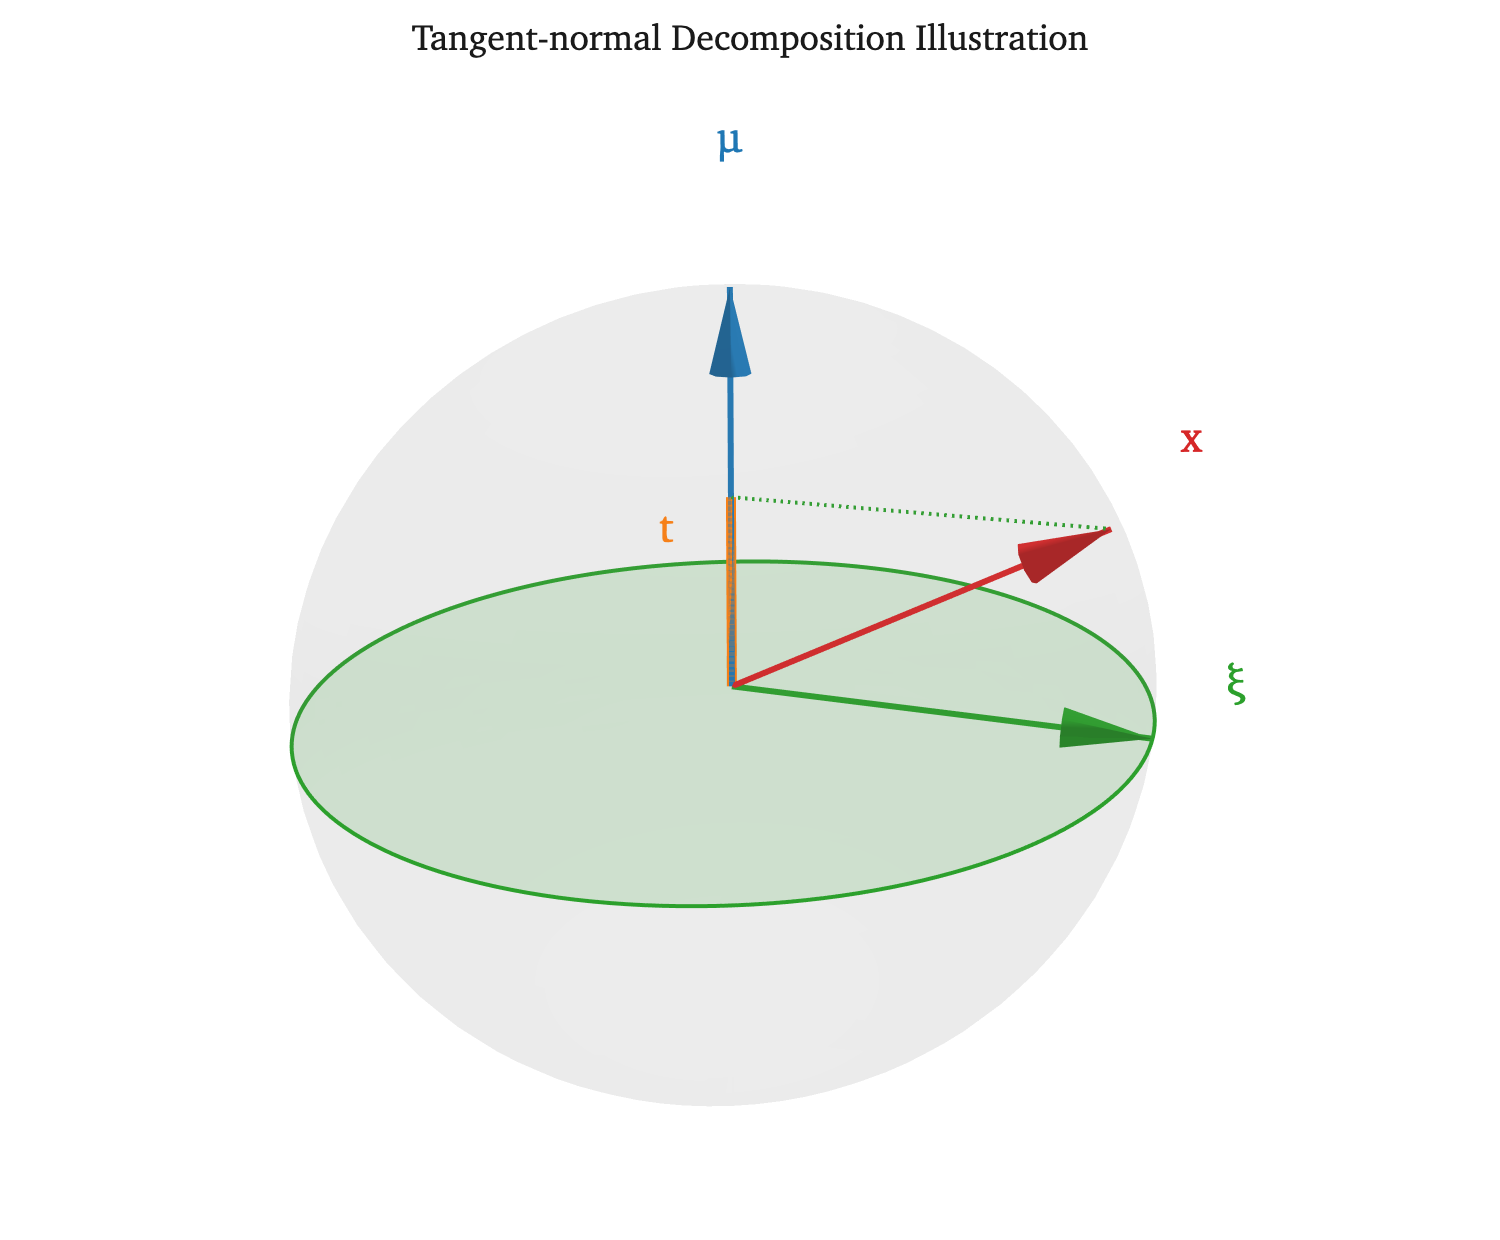
\includegraphics[trim=289 133 254 23, clip, width=\textwidth]{assets/tangent_normal_decomposition.png}
    \label[figure]{fig:tangent-normal-illustration}
\end{minipage}

The statements and intuition that follow are largely introduced in \cite{decao2020powersphericaldistribution} and
\cite{mardia2009directional}.
\begin{theorem}[Marginal density of rotationally-symmetric distributions]
\label{thm:marginal}
Consider the tangent-normal decomposition of a unit vector $\mathbf{x} \in \mathbb{S}^{d - 1}$. The Lebesgue density of
$t = \boldsymbol{\mu}^\top\mathbf{x}$ is given by
\[
    \sigma_t = B\left(\frac{d - 1}{2}, \frac{1}{2}\right)^{-1}\left(1 - t^2\right)^{\frac{d - 3}{2}}
\]
Consequently, if $f(\mathbf{x}; \boldsymbol{\mu}, \boldsymbol{\Theta})$ is a rotationally-symmetric distribution on the
unit hypersphere, it may be written in terms of its \textit{angular density} \citep{Garc_a_Portugu_s_2019} $g\left(\boldsymbol{\mu}^\top\mathbf{x}; \boldsymbol{\Theta}\right)$:
\[
    f(\mathbf{x}; \boldsymbol{\mu}, \boldsymbol{\Theta}) = \frac{g\left(\boldsymbol{\mu}^\top\mathbf{x}; \boldsymbol{\Theta}\right)}{\sigma_t}
\]
Additionally, $g$ may be written as
\[
    g\left(t; \boldsymbol{\Theta}\right) = C_T(\boldsymbol{\Theta})\phi(t; \boldsymbol{\Theta})\sigma_t
\]
where $C_T(\cdot)$ is a normalizing constant.
\end{theorem}
It thus suffices to consider rotationally-symmetric distributions on the unit hypersphere by their respective $\phi(t; \boldsymbol{\Theta})$ as
in \Cref{thm:marginal}. For the sake of brevity, we refer to these identifiers as \textit{angular kernels}.
\begin{example}
The \textit{von Mises-Fisher} (vMF) distribution with mean direction $\boldsymbol{\mu}$ and concentration $\kappa$ is a
rotationally-symmetric distribution with angular kernel $\phi(t; \kappa) = \exp(\kappa t)$. The full density is given by
\[
    f(\mathbf{x}; \boldsymbol{\mu}, \kappa) = \frac{\kappa^{\frac{d}{2} - 1}}{(2\pi)^{\frac{d}{2}}I_{\frac{d}{2} - 1}(\kappa)}\exp\left(\kappa\boldsymbol{\mu}^\top\mathbf{x}\right)
\]
as outlined in \cite{davidson2022hypersphericalvariationalautoencoders}, where $I_v$ denodes the modified Bessel function at
order $v$.
\end{example}
\begin{example}
The \textit{power-spherical} distribution \citep{decao2020powersphericaldistribution} with mean direction $\boldsymbol{\mu}$ and concentration $\kappa$ is a
rotationally-symmetric distribution with angular kernel $\phi(t; \kappa) = (1 + t)^\kappa$. The full density is given by
\[
    f(\mathbf{x}; \boldsymbol{\mu}, \kappa) = \left[ 2^{\alpha + \beta}\pi^\beta \frac{\Gamma(\alpha)}{\Gamma(\alpha + \beta)} \right]^{-1}\left(1 + \boldsymbol{\mu}^\top\mathbf{x}\right)^\kappa, \qquad \alpha = \frac{d - 1}{2} + \kappa, \beta = \frac{d - 1}{2}
\]
Both the vMF and power-spherical distributions can be considered as ``location-scale'' distributions on the unit
hypersphere, almost as spherical analogues to the normal distribution. 
\end{example}
\begin{figure}[H]
    \centering
    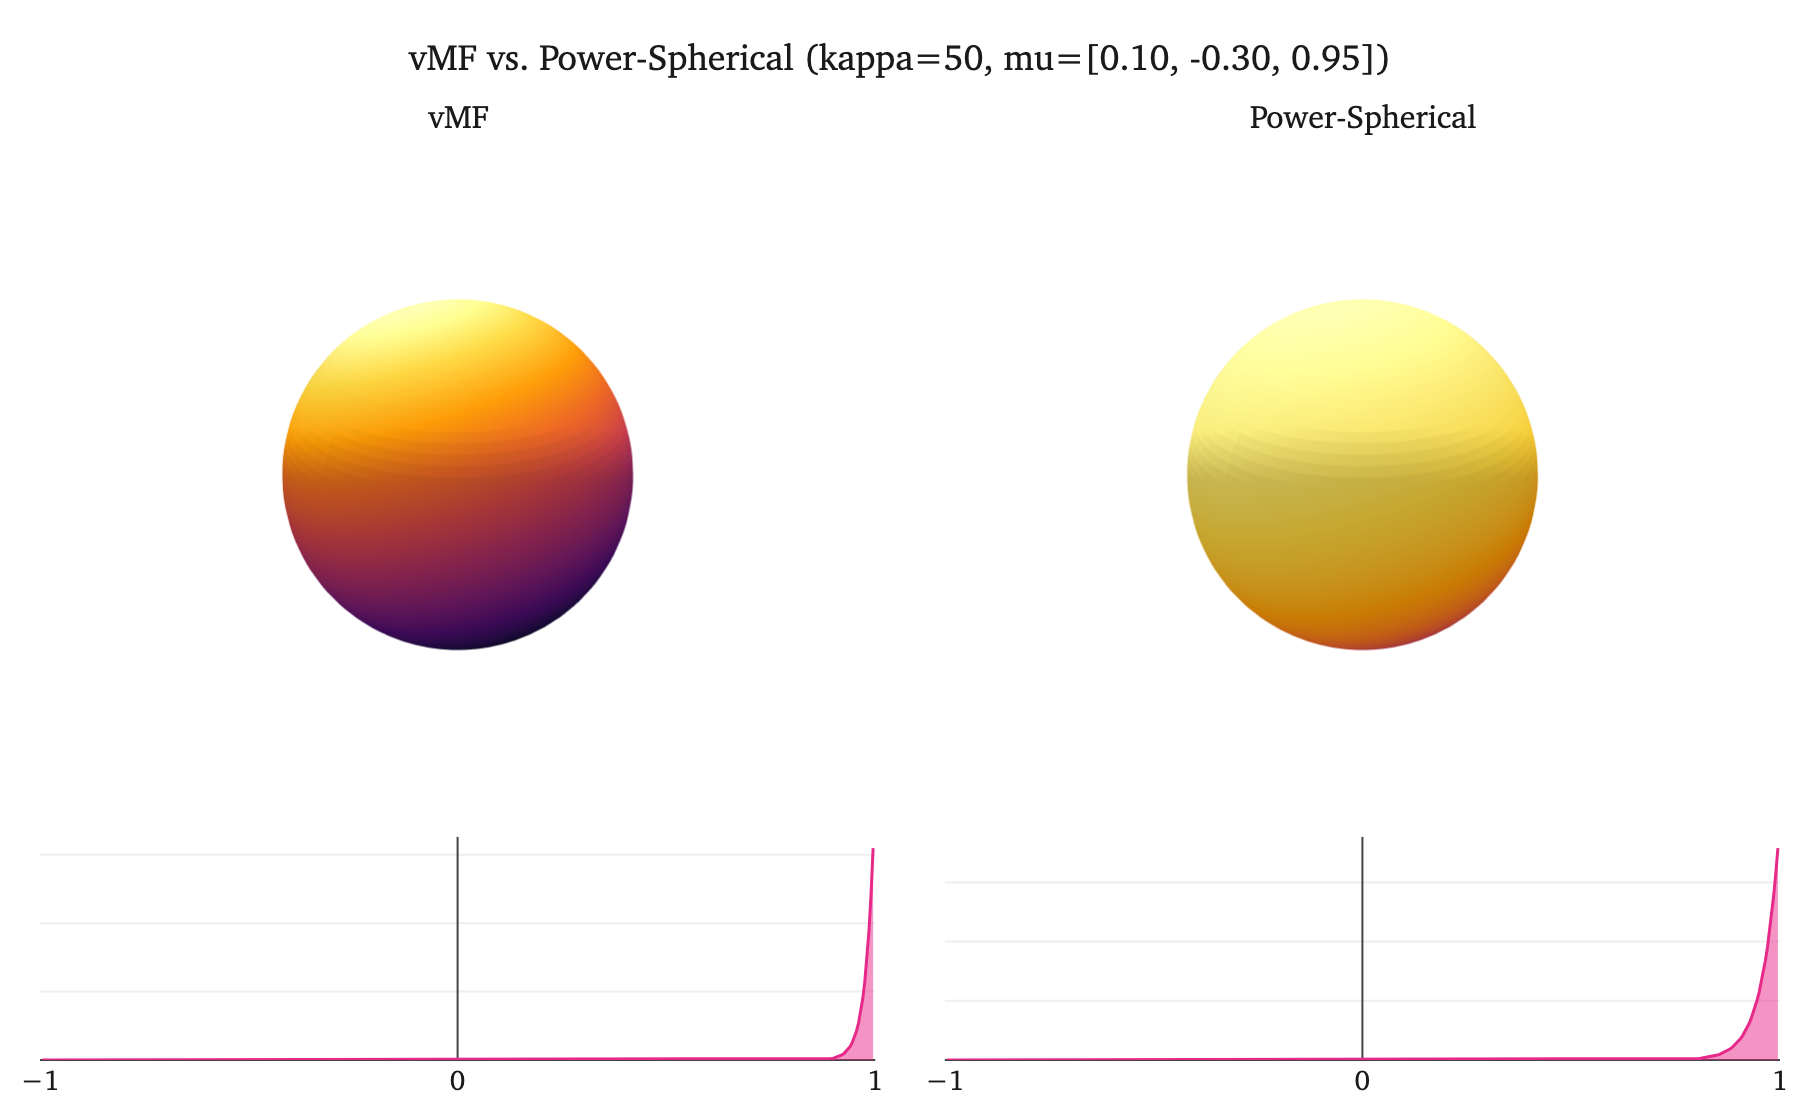
\includegraphics[width=\textwidth]{assets/location_scale_comparison.png}
    \caption{Von Mises-Fisher (left) and power-spherical (right) on $\mathbb{S}^2$ at the same mean direction
    $\boldsymbol{\mu} = (0.1, -0.3, 0.95)$ and the same concentration $\kappa = 50$: a log-density heatmap on the
    sphere above each family's univariate angular density $g(t; \kappa)$ below.}
    \label{fig:vmf-power-spherical-comparison}
\end{figure}
Aside from lighter tails, the power-spherical distribution distinguishes itself from the vMF distribution
through significantly faster sampling and numerically stable density evaluation. Since the vMF distribution's
angular density depends on the modified Bessel function, it does not admit an inverse CDF. As such, producing vMF samples
requires rejection sampling as outlined in \cite{davidson2022hypersphericalvariationalautoencoders}. The power-spherical
distribution, on the other hand, can be produced by a deterministic transformation of a beta-distributed sample:
\[
    X  = 2Z - 1, \qquad Z \sim \text{Beta}\left(\frac{d - 1}{2} + \kappa, \frac{d - 1}{2}\right)
\]
Above, $X$ follows the angular density of a power-spherical distribution. It is important to note, however, that both
of the above distributions are limited in their expressivity:
\begin{theorem}[Modality of the vMF and Power-Spherical Distributions]
\label{thm:locscale-modality}
For any mean direction $\boldsymbol{\mu} \in \mathbb{S}^{d - 1}$ and concentration $\kappa > 0$, the vMF and
power-spherical distributions are unimodal with unique mode at $\boldsymbol{\mu}$.
\end{theorem}
Below, we introduce a new distribution on the unit hypersphere which admits greater expressivity.


\section{The TNBBeta and SphericalTNBBeta Distributions}
The \textit{triply-randomized negative binomial beta} (TNBBeta) distribution \citep{lederman2026triplyrandomizednegativebinomialbeta}
is defined on the unit interval with the following density:
\begin{align*}
    \text{TNBBeta}(y; p, q, \varepsilon) &= \text{Beta}(\varepsilon, \varepsilon)\left[\frac{1 - q}{y(1 - y)}\gamma(y, p)\right]^{\varepsilon}\left[1 - 4q\gamma(y, p)\right]^{-\left(\varepsilon + \frac{1}{2}\right)} \\
    \gamma(y, p) &= \frac{1}{4}\operatorname{sech}^2\left(\frac{\operatorname{logit}(y) - \operatorname{logit}(p)}{2}\right)
\end{align*}
where $p \in (0, 1)$ governs the median, $q \in [0, 1)$ governs the concentration about $p$, and $\varepsilon > 0$
controls both concentration about $p$ and tail behavior of the distribution. By scaling a TNBBeta random variable to
the interval $[-1, 1]$ and applying \Cref{alg:tnbbeta-sample}, we are able to produce another rotationally-symmetric
distribution on the unit hypersphere, which we refer to as the SphericalTNBBeta distribution.

\Cref{fig:pq-ablation} and \Cref{fig:p-epsilon-ablation} illustrate some examples of the SphericalTNBBeta distribution over
$\mathbb{S}^2$.
\begin{figure}[H]
    \centering
    \begin{minipage}[t]{0.48\textwidth}
        \centering
        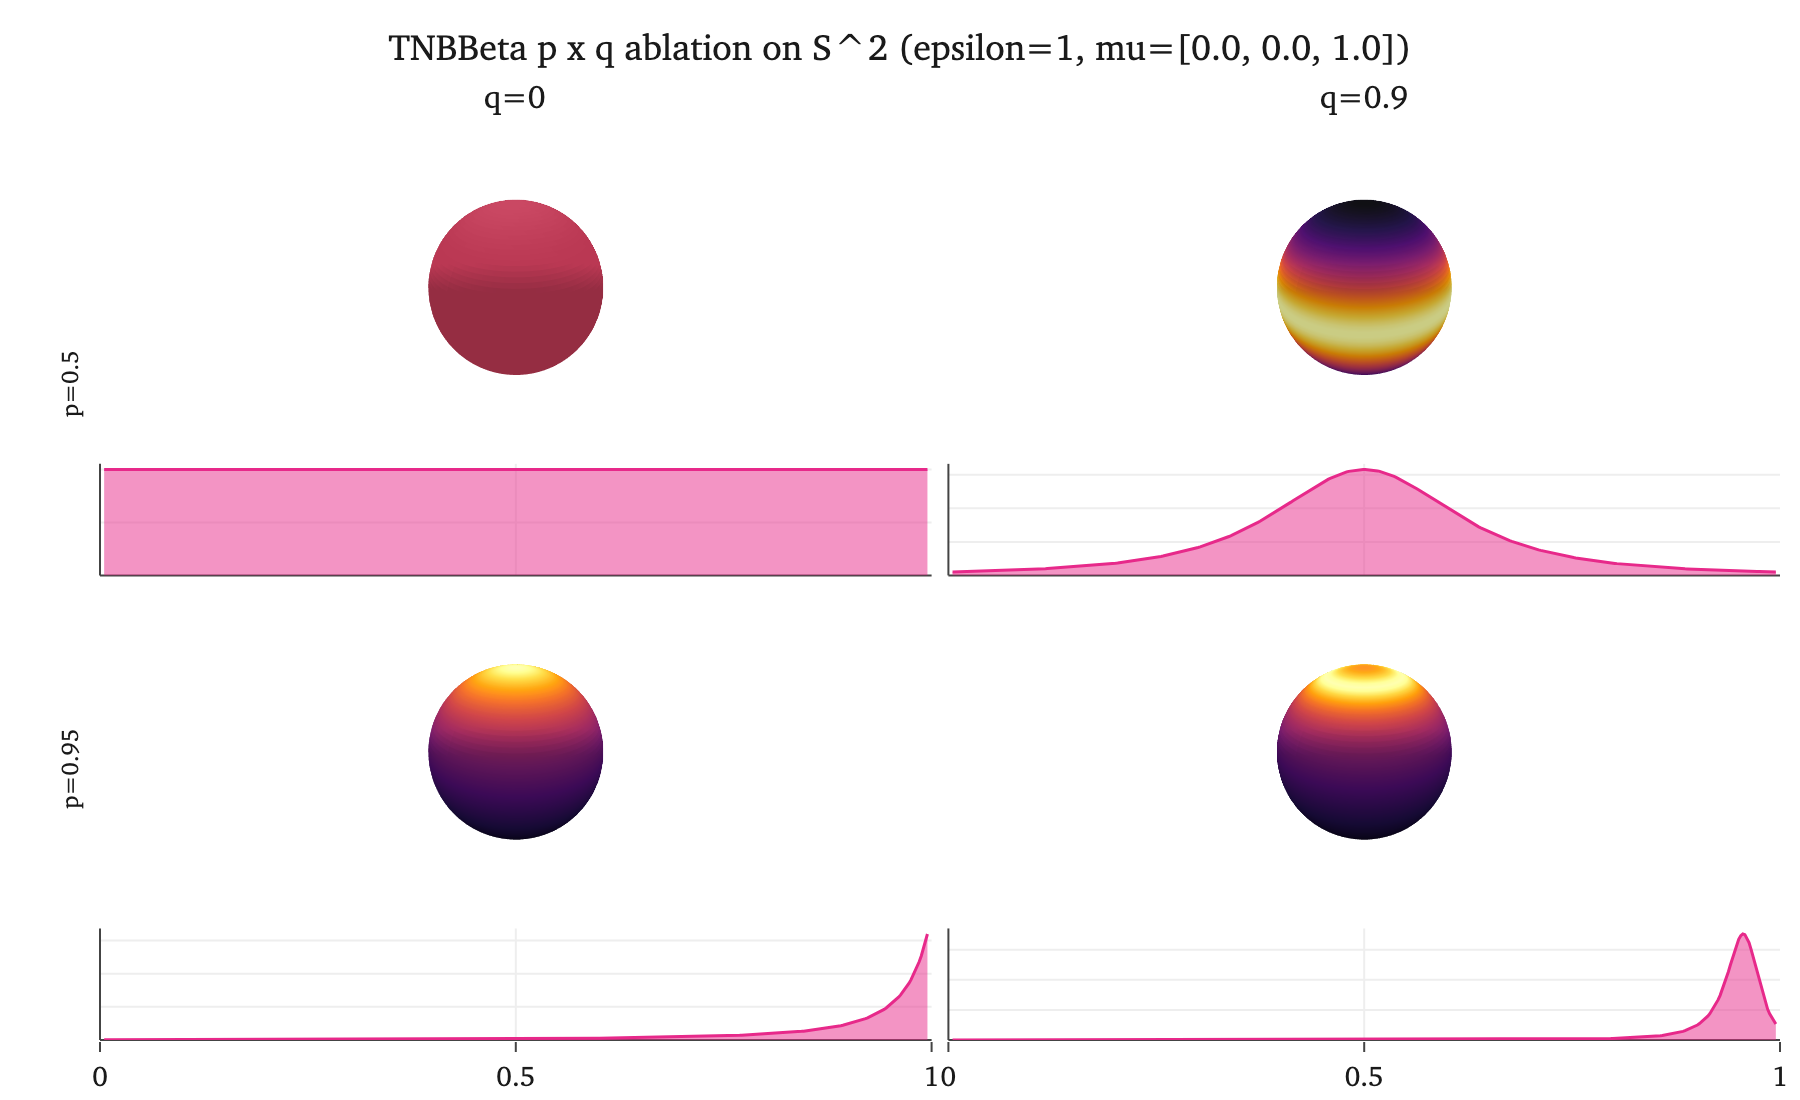
\includegraphics[width=\textwidth]{assets/pq_ablation_2x2.png}
        \captionsetup{width=\linewidth}
        \captionof{figure}{SphericalTNBBeta on $\mathbb{S}^2$ across $p \in \{0.5, 0.95\}$ and $q \in \{0, 0.9\}$
        ($\varepsilon = 1$ fixed): a log-density heatmap above its univariate density below.}
        \label{fig:pq-ablation}
    \end{minipage}
    \hfill
    \begin{minipage}[t]{0.48\textwidth}
        \centering
        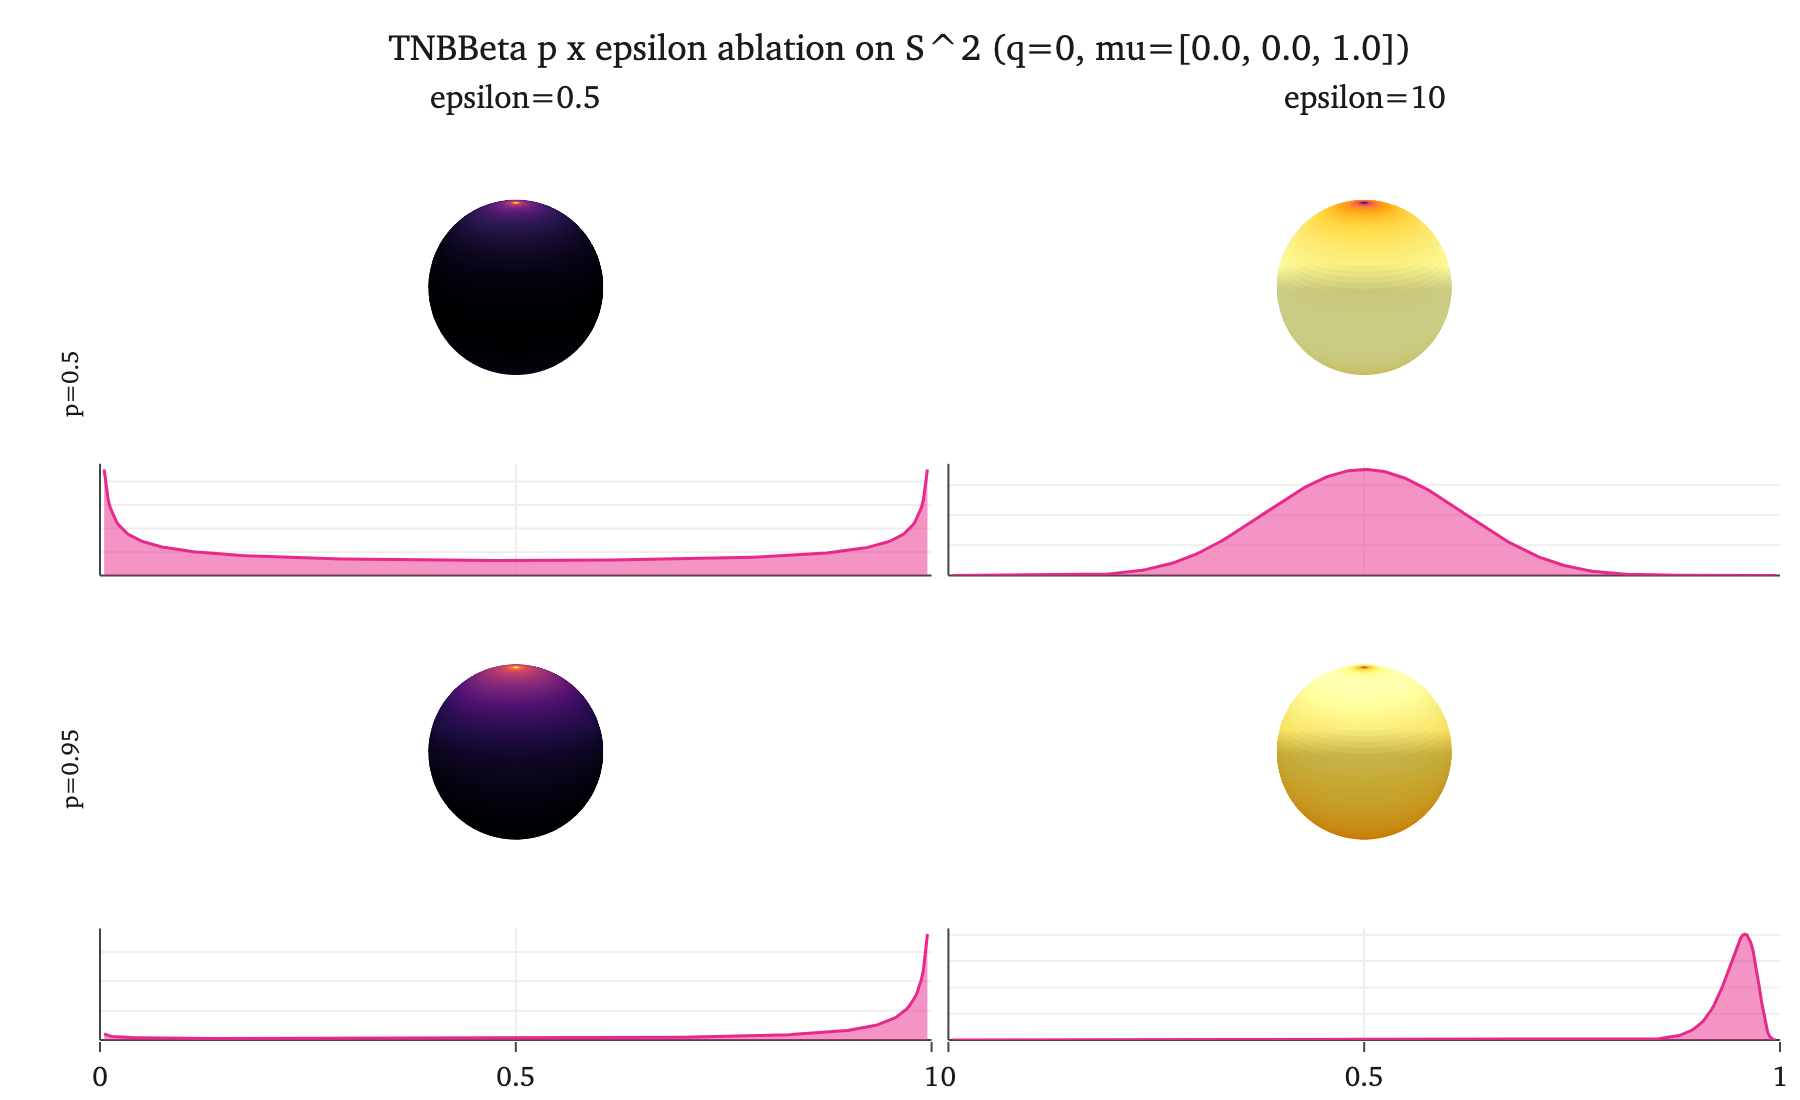
\includegraphics[width=\textwidth]{assets/p_epsilon_ablation_2x2.png}
        \captionsetup{width=\linewidth}
        \captionof{figure}{SphericalTNBBeta on $\mathbb{S}^2$ across $p \in \{0.5, 0.95\}$ and
        $\varepsilon \in \{0.5, 10\}$ ($q = 0$ fixed): $\varepsilon = 0.5$ shows antipodal bimodality,
        $\varepsilon = 10$ shows unimodal concentration.}
        \label{fig:p-epsilon-ablation}
    \end{minipage}
\end{figure}
The bottom-left heatmap of \Cref{fig:pq-ablation} closely resembles the cap-like shape of a vMF or
power-spherical distribution, and this resemblance holds, specifically as $p$ approaches 1:
\begin{theorem}[Limiting behavior of the SphericalTNBBeta distribution]
\label{thm:limiting-tnbbeta}
Suppose $\varepsilon > (d - 1) / 2$. As $p \to 1$, the $\mathrm{SphericalTNBBeta}(\mathbf{x}; \boldsymbol{\mu}, p, q, \varepsilon)$
distribution converges to a dirac mass about $\boldsymbol{\mu}$ and its mass is concentrated within $O(1 - p)$ of $\boldsymbol{\mu}$.
\end{theorem}
As \Cref{fig:pq-ablation} and \Cref{fig:p-epsilon-ablation} show, though, the SphericalTNBBeta distribution is capable of
expressing more shapes, as well as admitting two or more modes. This notion is formalized in \Cref{thm:modality-tnbbeta}.
\begin{theorem}[Modality of the SphericalTNBBeta distribution]
\label{thm:modality-tnbbeta}
For any $p \in (0, 1)$ and $q \in [0, 1)$,
\begin{itemize}
    \item If $\varepsilon > (d - 1) / 2$, $\mathrm{SphericalTNBBeta}(\mathbf{x}; \boldsymbol{\mu}, p, q, \varepsilon)$ is unimodal
    \item If $\varepsilon < (d - 1) / 2$, $\mathrm{SphericalTNBBeta}(\mathbf{x}; \boldsymbol{\mu}, p, q, \varepsilon)$ has at least
    two modes, two of which are located at $\pm \boldsymbol{\mu}$
\end{itemize}
\end{theorem}
Finally, it is important to note that the TNBBeta distribution can be sampled via a deterministic transformation of a single beta-distributed
sample. Hence, given a more expressive density shape, as well as the ability to employ gradient reparametrization, the
SphericalTNBBeta makes for an interesting choice of posterior for a hyperspherical variational autoencoder.

\section{Experiments}
Since the SphericalTNBBeta distribution does not require rejection sampling, it admits significantly
faster sampling than the vMF distribution:
\begin{figure}[H]
    \centering
    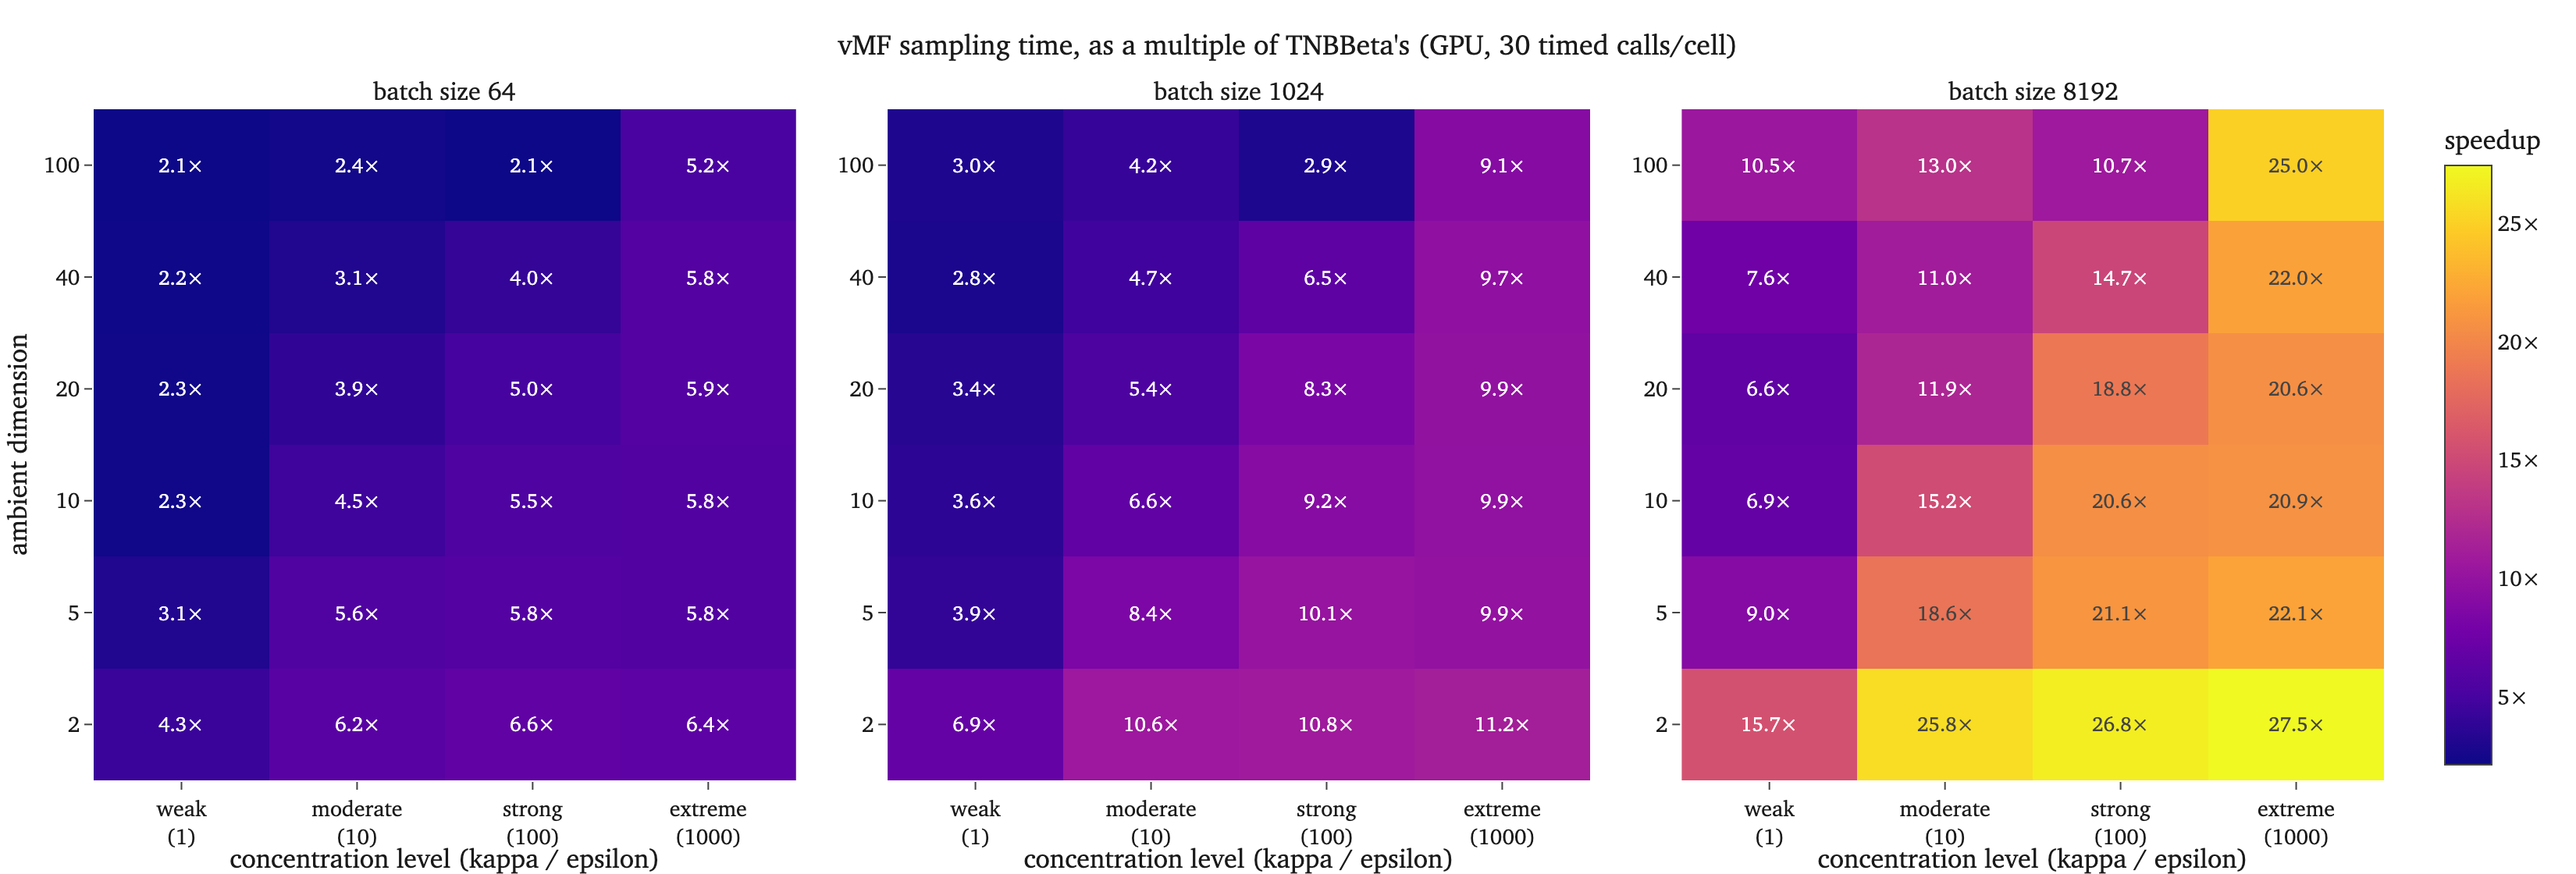
\includegraphics[width=\textwidth]{assets/sampling_speed_heatmap.png}
    \caption{Comparison between sampling time for a single SphericalTNBBeta batch and a single vMF batch on one GPU}
\end{figure}
At the $d=64$ level it is worth noting that this speedup is comparable to that of the power-spherical distribution,
as outlined in Figure 2b of \cite{decao2020powersphericaldistribution}. Given more recent deep generative
models tend to employ larger batch sizes on the order of $10^3$, we additionally included results for higher batch sizes
and note that the speedup is even more pronounced in those cases.

Sampling speed aside, we find that TNBBeta-VAE performance is nearly identical that of the power spherical VAE and the S-VAE, using
binarized MNIST \citep{lecun1998mnist} as a simple example.
\begin{figure}[H]
    \centering
    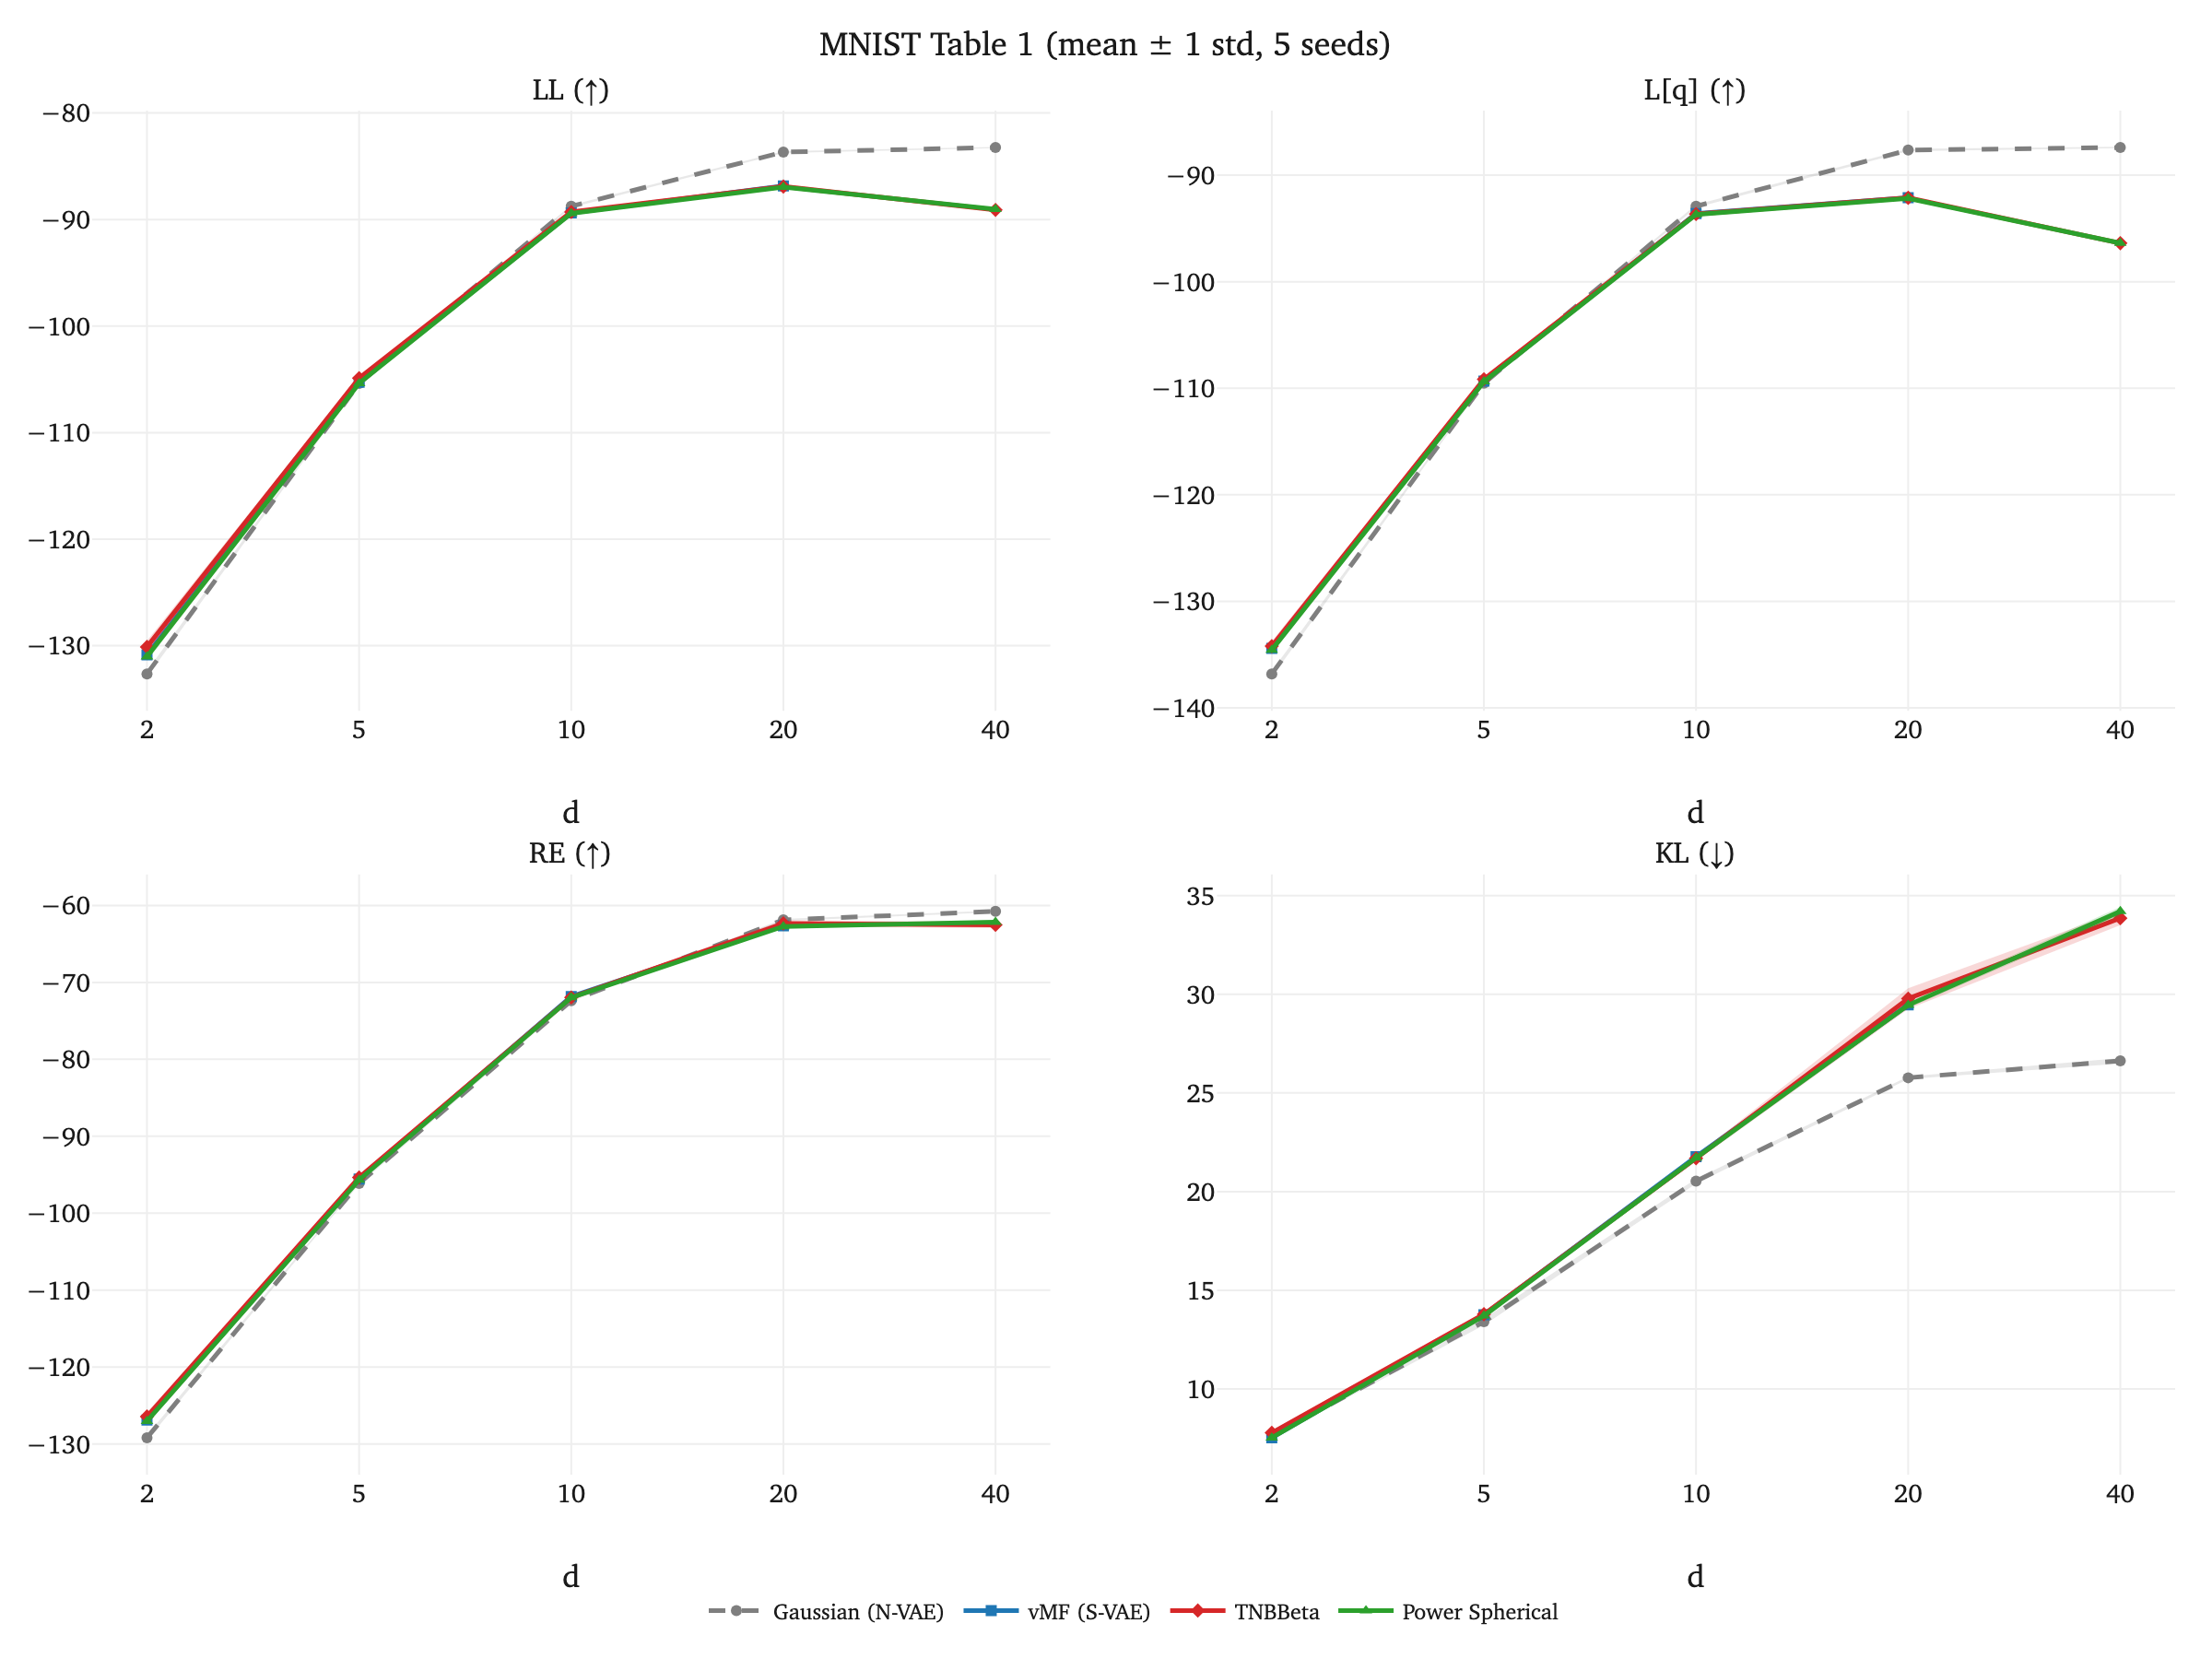
\includegraphics[width=\textwidth * 6 / 8]{assets/mnist_table1_lines.png}
    \caption{MNIST reconstruction quality, mean $\pm 1$ standard deviation over 5 seeds}
    \label{fig:mnist-table1-lines}
\end{figure}
The above result is rather unsurprising once we consider the structure of the latent space for the S-VAE and TNBBeta-VAE.
\begin{figure}[H]
    \centering
    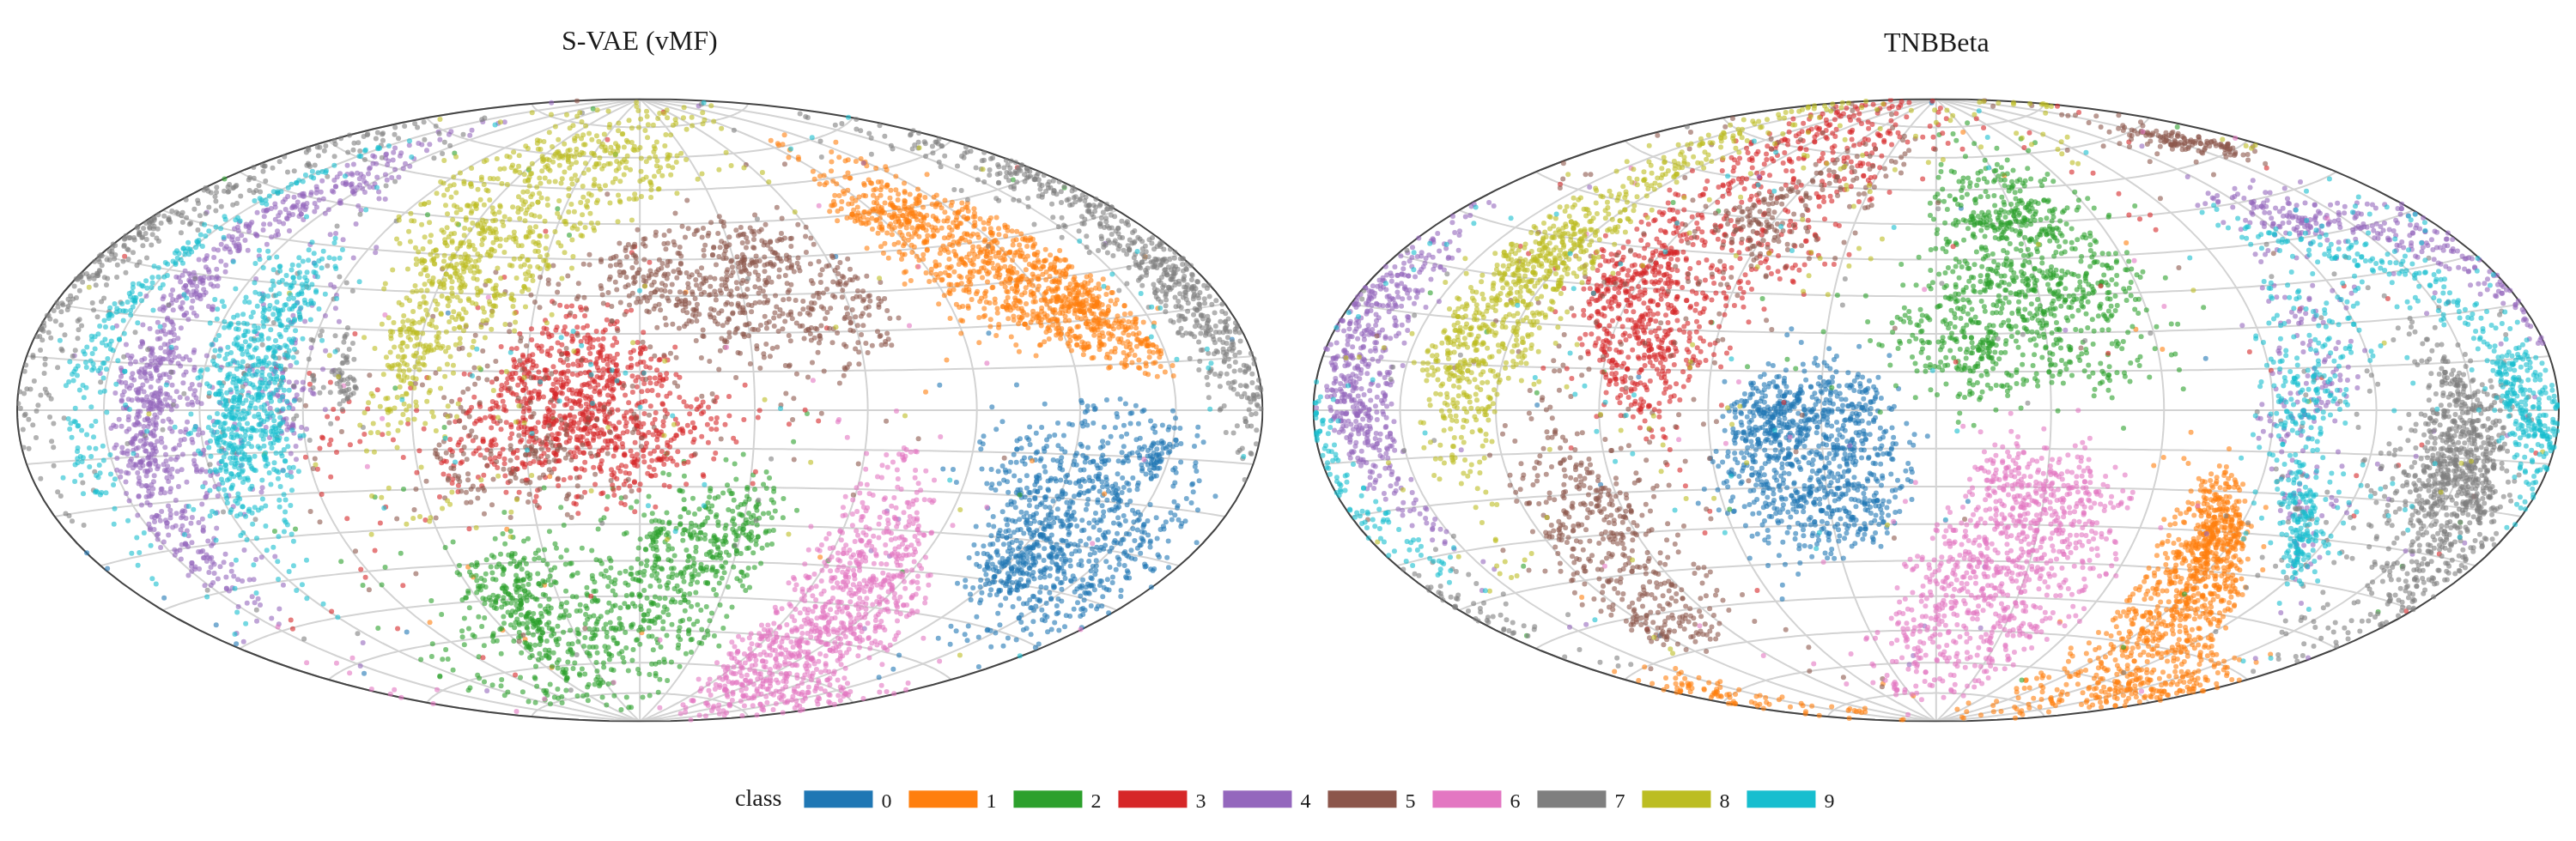
\includegraphics[width=\textwidth]{assets/hammer_mnist_vmfs_d2_seed0_vs_mnist_tnbs_d2_seed0.png}
    \caption{Hammer projection of MNIST embeddings in $\mathbb{S}^2$}
    \label{fig:hammer}
\end{figure}
\Cref{fig:hammer} illustrates that the vMF and TNBBeta latent spaces both form cap-like structures around the unit hypersphere
in low dimensions, and \Cref{thm:limiting-tnbbeta} shows that, as $p \to 1$, this similarity in shape holds for higher
dimensions. \Cref{fig:appx-posterior-traj} shows that this asymptotic limit is indeed reached during training for various
latent dimensions.

One is then left to wonder where these posteriors diverge in shape. Variational graph autoencoders (VGAEs) \citep{kipf2016variationalgraphautoencoders}
provide one avenue to explore such differences. We trained a series of VGAEs on citation networks,
namely Cora, Pubmed, Citeseer \cite{https://doi.org/10.1609/aimag.v29i3.2157}, and computer science
coauthorship networks from the Microsoft Academic Graph, as constructed in \cite{shchur2019overlappingcommunitydetectiongraph}. For each dataset
and posterior approximation, we trained two VGAEs: one using the training adjacency matrix and individual node features, and one without
individual node features. After training, we evaluated link prediction AUC and AP on a held-out set of edges.
\Cref{fig:features-onoff-bars} shows that link prediction performance is indistinguishable between all posterior families
with node features, while Gaussian and SphericalTNBBeta posteriors dominate without node features.
\begin{figure}[H]
    \centering
    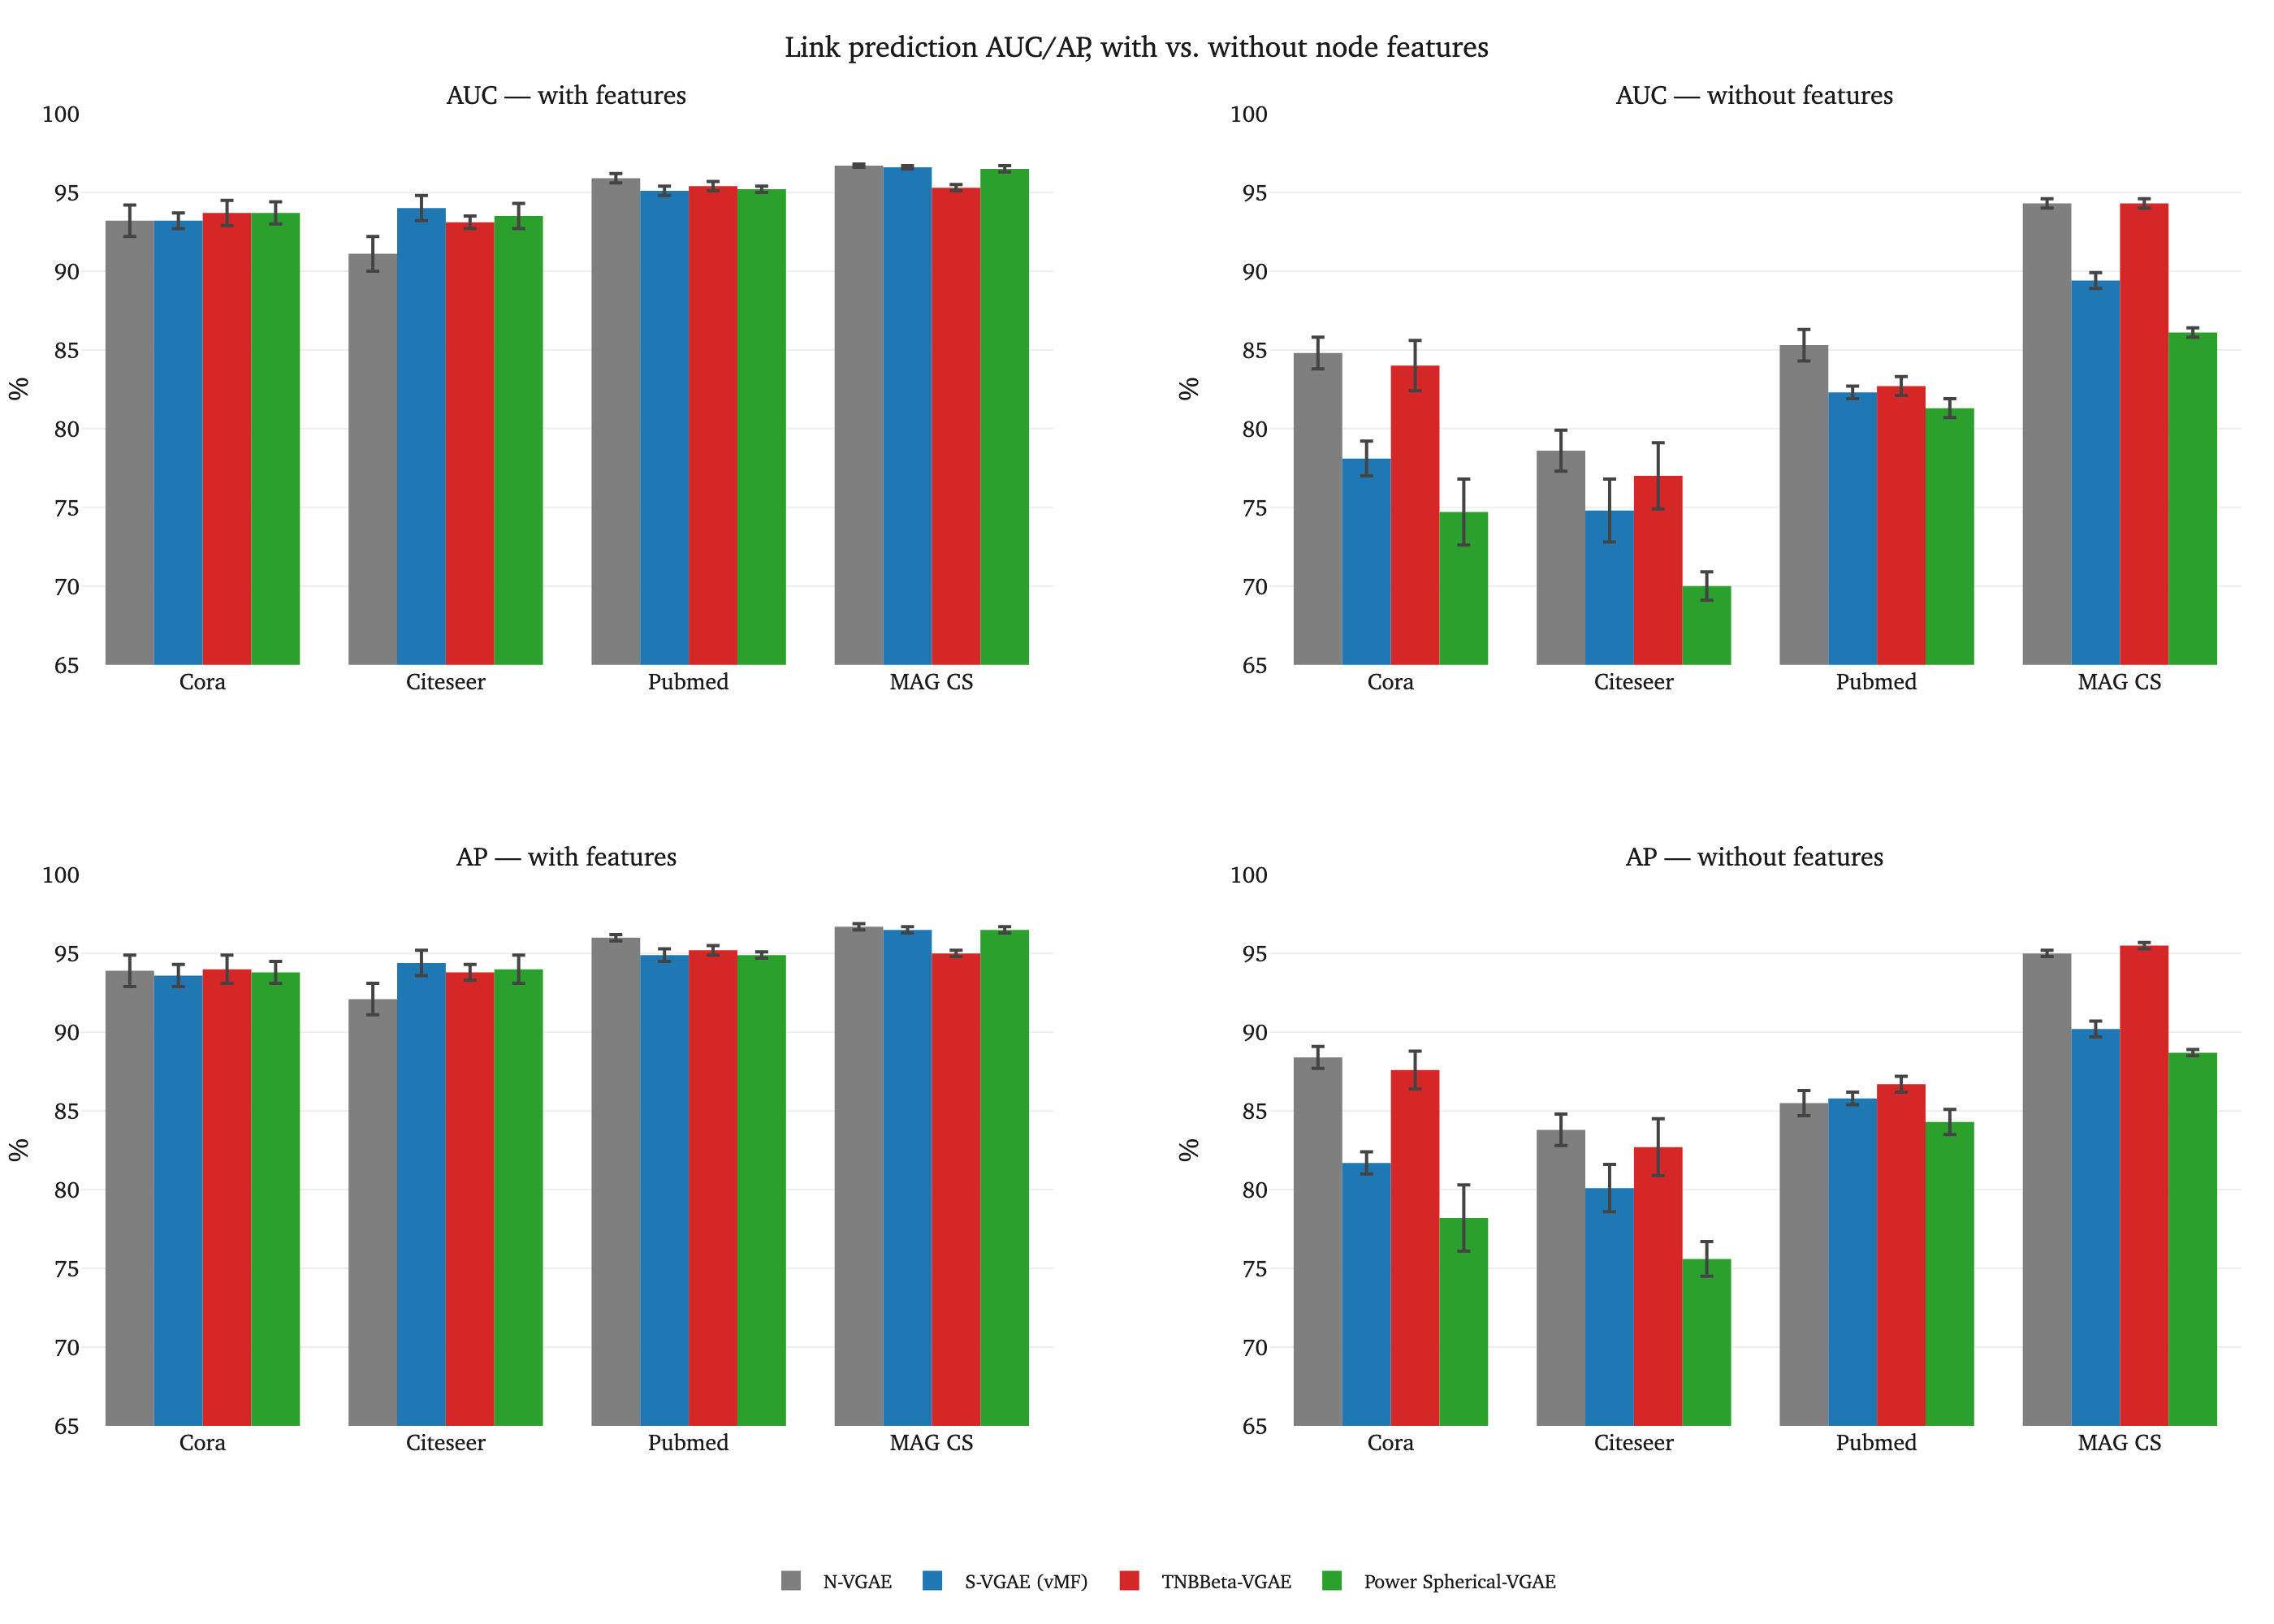
\includegraphics[width=\textwidth]{assets/features_onoff_bars.png}
    \caption{Link-prediction AUC (top) and AP (bottom), with features (left) vs.\ without (right), mean
    $\pm 1$ standard deviation over 5 seeds}
    \label{fig:features-onoff-bars}
\end{figure}

\Cref{fig:appx-posterior-traj} in appendix B shows that, in the MNIST experiments, the posterior $\varepsilon$ parameter always landed
in a unimodal regime (see \Cref{thm:modality-tnbbeta}). Let $m$ denote that threshold. In the above graph representation experiments,
we found $m$ to be consistently within a \textit{bimodal} regime. To understand what node characteristics affect the modality of
the per-point posterior, we constructed a series of synthetic graphs. Each graph contains ten communities, with 50 nodes per community.
We assign each graph a probability $p_{\text{out}}$, and construct the adjacency matrix $A_{ij} \sim \text{Bernoulli}(p_{\text{out}})$
if nodes $i$ and $j$ do not share a community. Otherwise, we draw $A_{ij} \sim \text{Bernoulli}(0.3)$.
\begin{figure}[H]
    \centering
    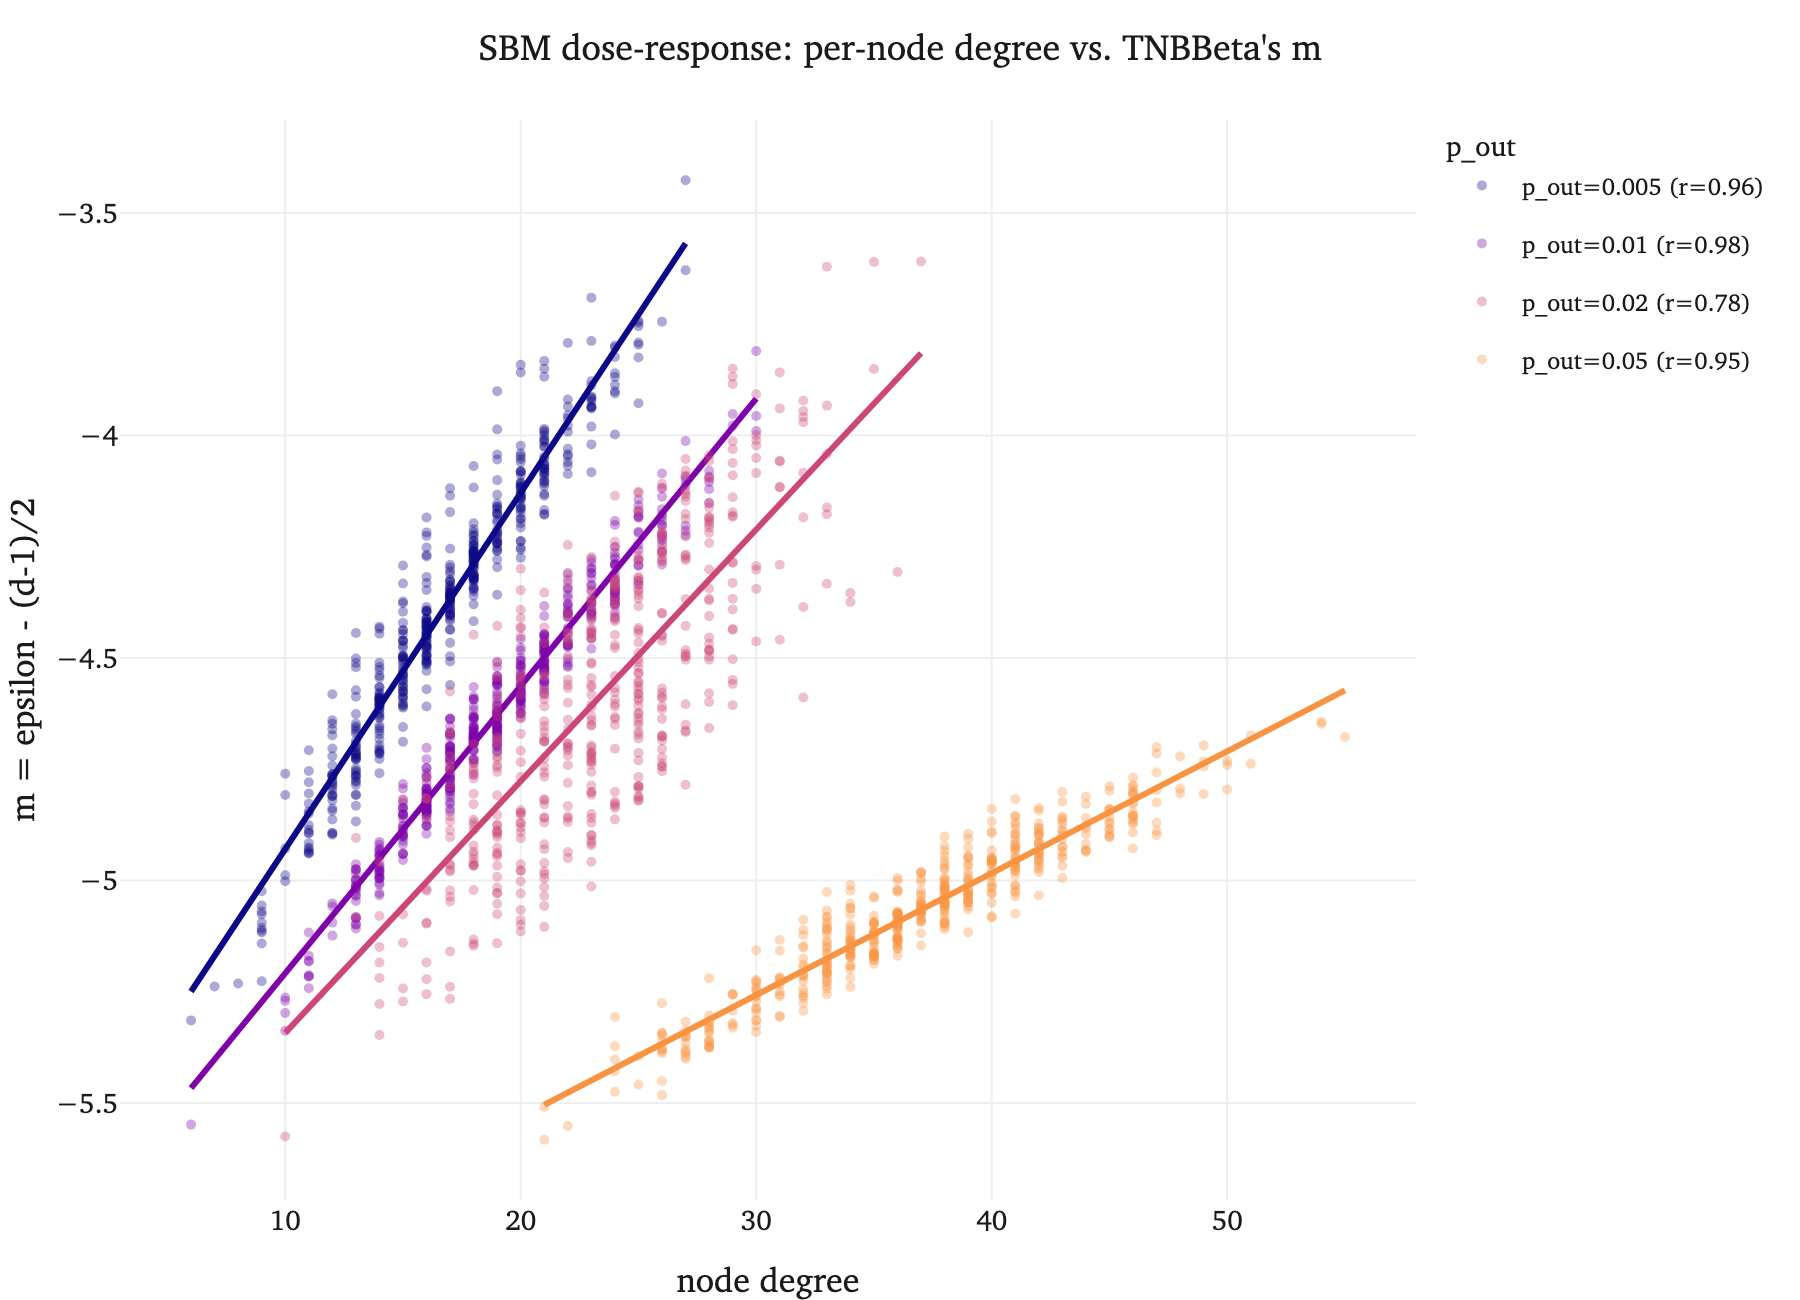
\includegraphics[width=\textwidth * 6 / 8]{assets/sbm_degree_vs_m.png}
    \caption{Per-node degree vs.\ $m$ on the synthetic graphs, one color per $p_{\text{out}}$ level, with
    a line of best fit and Pearson $r$ per level.}
    \label{fig:sbm-degree-vs-m}
\end{figure}
We find that, on average, as $p_{\text{out}}$ increases, $m$ becomes \textit{more} negative. Namely, multimodality
correlates with how densely-connected the graph's \textit{communities} are. What is more interesting, and yet to be explored,
is that $m$ and $\text{deg}(i)$ are \textit{positively} correlated\footnote{We omit the results for $p = 0.1$ as those produced a constant value of $m$. This is yet to be investigated.}. One would expect that nodes with high degree and thus a higher
chance of links to several other communities take greater advantage of multimodality. The above, in fact, shows the opposite.

\section{Conclusion}
We presented an overview of approaches to VAEs on the unit hypersphere using rotationally-symmetric
distributions as posterior approximations. To introduce greater flexibility, we introduced the
SphericalTNBBeta distribution which is able to admit a bimodal structure that neither the vMF nor the
power-spherical distributions can attain. We showed that performance of VAEs trained with these posteriors
nearly match on tasks as simple as MNIST, while the SphericalTNBBeta takes a clear lead on link prediction
performance for featureless graphs.

\section*{Acknowledgements}
I would like to thank Aaron Schein and Jimmy Lederman for their invaluable help, advice,
and insight throughout the process of writing this paper.

\section*{Generative AI Attestation}
Generative AI (specifically, Claude Sonnet 5) was used in the generation of all code to assist
with running the above experiments, as well as generating the above visualizations. It was
additionally used to assist with proof-reading the proofs of theorems 2.4 and 3.2, as well as
helping with a sketch of theorem 3.1. I assert that I have reviewed the above results and claim
responsibility for the above statements. All commentary in the writeup aside from the captions
is my own. So is all analysis above.


\appendix
\section{Proofs}
\begin{proof}[Proof of \Cref{thm:marginal}]
The construction of $\sigma_t$ comes from 9.3.1 of \cite{mardia2009directional}. The remainder follows directly, as
the vector $\boldsymbol{\xi}$ is uniformly distributed on $\mathbb{S}^{d - 2}$ and independent of $t$.
\end{proof}

\begin{proof}[Proof of \Cref{thm:locscale-modality}]
This largely follows from definitions 1 and 2 of \cite{decao2020powersphericaldistribution}.
Fix $\boldsymbol{\mu} \in \mathbb{S}^{d - 1}, \kappa > 0$. The unnormalized vMF and power-spherical densities
are given by
\[
    p_{\text{vMF}}(\mathbf{x}; \boldsymbol{\mu}, \kappa) \propto \exp\left\{ \kappa\boldsymbol{\mu}^\top\mathbf{x} \right\}
    , \quad
    p_{\text{PS}}(\mathbf{x}; \boldsymbol{\mu}, \kappa) \propto \left(1 + \boldsymbol{\mu}^\top\mathbf{x}\right)^\kappa
\]
Since $\kappa > 0$, observe that $\exp$ and $y \mapsto y^\kappa$ are monotone increasing in $\boldsymbol{\mu}^\top\mathbf{x}$,
which is uniquely maximized (equal to 1) by $\mathbf{x} = \boldsymbol{\mu}$. Hence, both densities admit a unique mode at
$\mathbf{x} = \boldsymbol{\mu}$.
\end{proof}

\begin{proof}[Proof of \Cref{thm:modality-tnbbeta}]
We may proceed closely as in the proof of proposition 3.1 of \cite{lederman2026triplyrandomizednegativebinomialbeta}, and write
\[
    f(y) \defeq \mathrm{SphericalTNBBeta}(y; \boldsymbol{\mu}, p, q, \varepsilon) = \text{Beta}(y; \varepsilon, \varepsilon)\left[y(1 - y)\right]^{-\left(\frac{d - 3}{2}\right)}h(y)
\]
The function $h$ above is continuous, strictly positive, and bounded on $[0, 1]$, as argued in proposition 3.1.
We now consider a slightly modified kernel:
\[
    K(y) = \frac{1}{B(\varepsilon, \varepsilon)}\left[y(1 - y)\right]^{\varepsilon - \frac{d - 1}{2}}
\]
The remainder of the proof is almost identical to that of proposition 3.1, with the exception that we now consider
the cases $\varepsilon > (d - 1)/2$, $\varepsilon = (d - 1)/2$, and $\varepsilon < (d - 1)/2$.
\end{proof}

\begin{proof}[Proof of \Cref{thm:limiting-tnbbeta}]
Consider the family of random variables $\{Z_p\}_{p \in (0, 1)}$ where
\[
Z_p \sim \mathrm{SphericalTNBBeta}(\boldsymbol{\mu}, p, q, \varepsilon)
\]
We know that for each $p$, the latitude $Y_p$ is distributed $\mathrm{TNBBeta}(p, q, \varepsilon)$. Let
$T_p \defeq (1 - Y_p)/(1 - p) = (1 - Y_p)/\delta$. It suffices to show that the family $\{T_p\}$ is tight.
By change of variables, the density for $T_p$ is given by
\begin{align*}
    f_{\delta}(t) &= \delta\frac{(1 - \delta t)^{\varepsilon - 1}(\delta t)^{\varepsilon - 1}}{B(\varepsilon, \varepsilon)}\left[\frac{1 - q}{(1 - \delta t)\delta t}\gamma\right]^{\varepsilon}\left[1 - 4q\gamma\right]^{-\left(\varepsilon + \frac{1}{2}\right)} \\
    &= \frac{1}{t(1 - \delta t)B(\varepsilon, \varepsilon)}\left[(1 - q)\gamma\right]^{\varepsilon}\left[1 - 4q\gamma\right]^{-\left(\varepsilon + \frac{1}{2}\right)} \\
    &= \frac{(1 - q)^{\varepsilon}}{B(\varepsilon, \varepsilon)} \cdot \left[1 - 4q\gamma\right]^{-\left(\varepsilon + \frac{1}{2}\right)} \cdot \frac{\gamma^{\varepsilon}}{t(1 - \delta t)} 
\end{align*}
Because of the $\operatorname{sech}$ term, it follows that $\gamma \leq 1/4$ regardless of the value of $\delta$. We then see that
\begin{align*}
    f_{\delta}(t) &\leq \frac{(1 - q)^{\varepsilon}}{B(\varepsilon, \varepsilon)}(1 - q)^{-\left(\varepsilon + \frac{1}{2}\right)}\frac{\gamma^{\varepsilon}}{t(1 - \delta t)} = \frac{1}{\sqrt{1 - q}B(\varepsilon, \varepsilon)}\frac{\gamma^{\varepsilon}}{t(1 - \delta t)}
\end{align*}
Now, we rewrite $\gamma$:
\begin{align*}
    \gamma &= \frac{\delta t(1 - \delta t)(1 - \delta)\delta}{\left[(1 - \delta)\delta t + \delta(1 - \delta t)\right]^2} = \frac{t(1 - \delta t)(1 - \delta)}{\left[t(1 - \delta) + 1 - \delta t\right]^2}
\end{align*}
and we can see that for $\delta < 1/2$,
\[
    \frac{1}{\left[t(1 - \delta) + 1 - \delta t\right]^2} \leq \frac{1}{\left[1 + t(1 - 2\delta)\right]^2} \leq \frac{1}{\left[1 + ct\right]^2} \leq \frac{4}{t^2}
\]
Using the fact that $(1 - \delta) < 1$ we bound $\gamma$ above as
\[
    \gamma \leq \frac{4(1 - \delta t)}{t}
\]
Hence, substituting this inequality for $\gamma$ back into $f_{\delta}$ yields
\[
    f_{\delta}(t) \leq \underbrace{\frac{4^{\varepsilon}}{\sqrt{1 - q}B(\varepsilon, \varepsilon)}}_{K}t^{-\varepsilon - 1}(1 - \delta t)^{\varepsilon - 1} \leq Kt^{-\varepsilon - 1}
\]
It then follows that for any $\zeta > 0$, choose $M = (\zeta K/\varepsilon)^{(1/\varepsilon)}$ such that
\[
    \mathbb{P}\left\{T_p > M\right\} \leq K\int_M^{1/\delta} t^{-\varepsilon - 1}\mathrm{d}t < K\int_M^{\infty} t^{-\varepsilon - 1}\mathrm{d}t = \frac{K}{\varepsilon M^{\varepsilon}} = \zeta
\]
and so the family $\{T_p\}$ is tight since $p$ was chosen arbitrarily above.

It immediately follows from tightness of $T_p$ that $Z_p$ is concentrated within $O(1 - p)$ about $\boldsymbol{\mu}$.
Now, we see that for any $\zeta$, as $p \to 1$,
\[
    \mathbb{P}\left\{1 - Y_p > \zeta\right\} = \mathbb{P}\left\{T_p > \frac{\zeta}{1 - p}\right\} \to 0
\]
It follows that $Y_p \to 1$ in probability, and thus $Z_p \to \boldsymbol{\mu}$ in probability.
\end{proof}

\section{Additional Visualizations}
\begin{figure}[H]
    \centering
    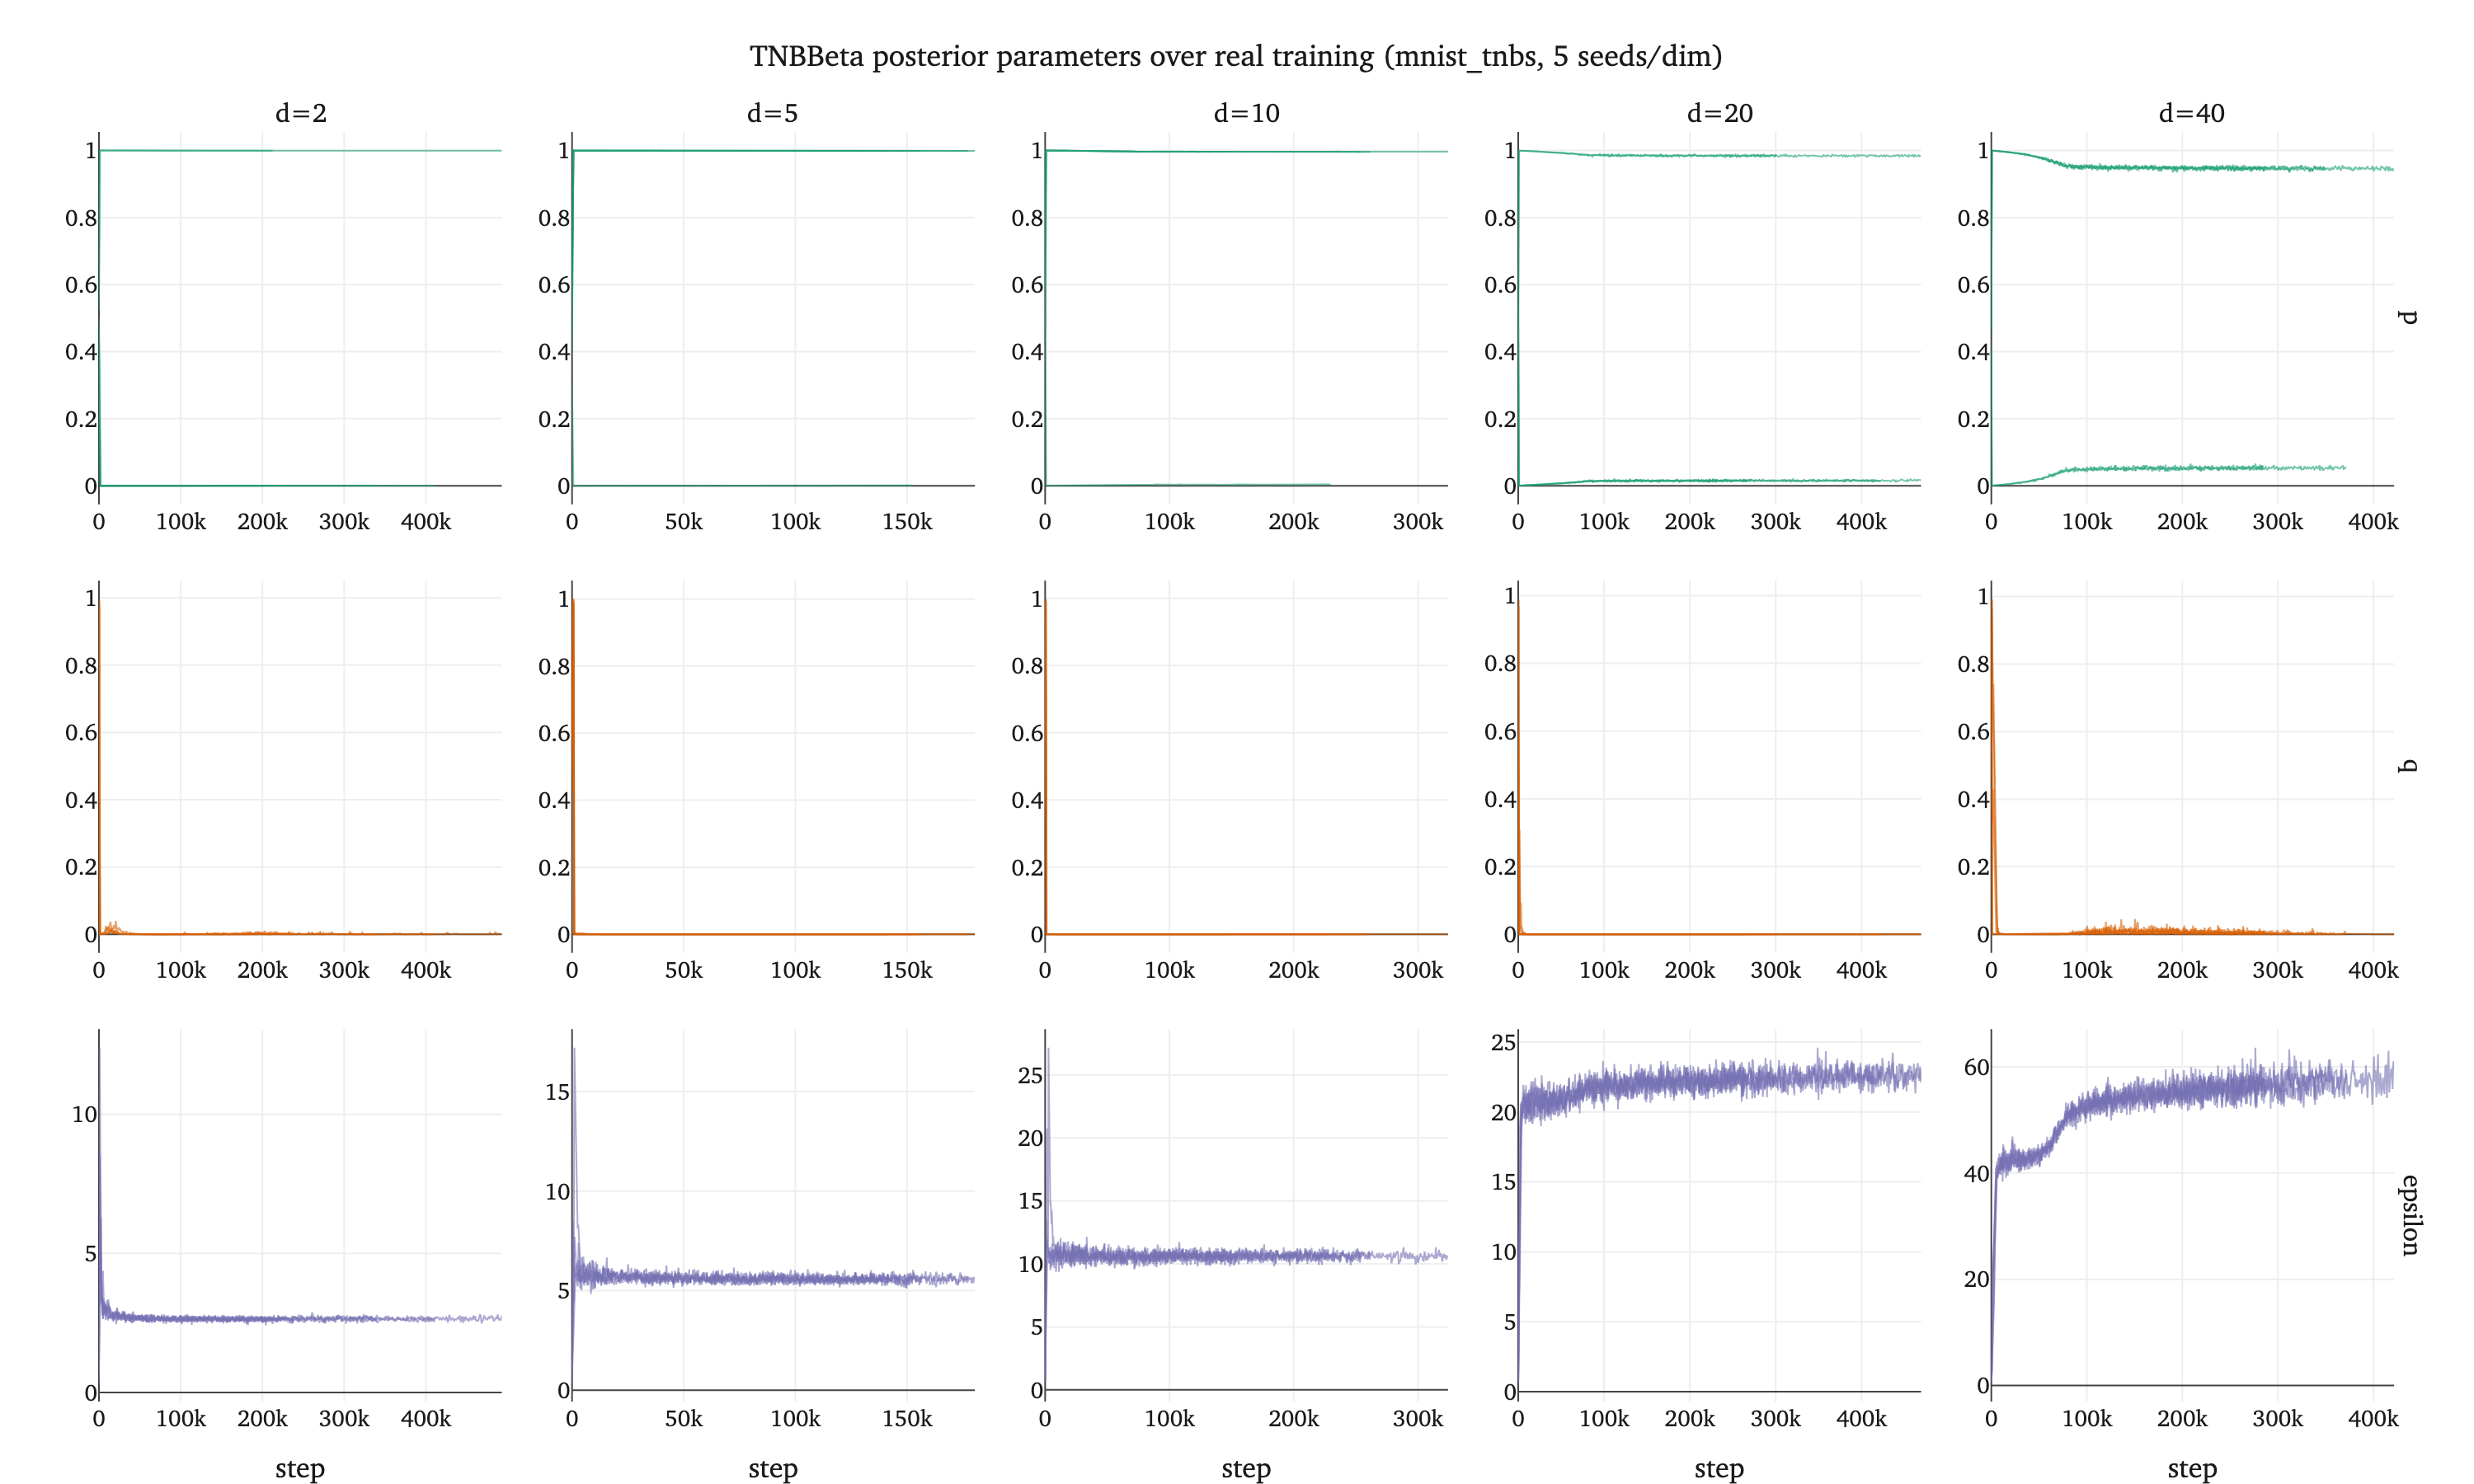
\includegraphics[width=\textwidth]{assets/tnbbeta_posterior_trajectories.png}
    \caption{Training trajectories of SphericalTNBBeta parameters on MNIST}
    \label{fig:appx-posterior-traj}
\end{figure}

\bibliographystyle{plainnat}
\bibliography{references}

\end{document}
